
\documentclass[11pt,a4paper]{article}
\usepackage{geometry}
\geometry{a4paper,left=25mm,right=25mm, top=24mm, bottom=24mm}

\usepackage{amsmath,amssymb,amstext,amsthm}
\usepackage{optidef}
%\usepackage{ucs}
\usepackage[utf8x]{inputenc}
%\usepackage[T1]{fontenc}
\usepackage[ngerman]{babel}
%\usepackage[ngerman]{varioref}
\usepackage{xcolor}
\usepackage{babelbib}
\usepackage[hidelinks]{hyperref}

\usepackage{caption}
\usepackage[linesnumbered]{algorithm2e}
\usepackage{pgfplots}

\usepackage{tikz}
\usepackage{tikz-cd}


\DeclareMathOperator*{\Max}{max}
\newcommand{\N}{\mathbb{N}}
\newcommand{\Z}{\mathbb{Z}}
\newcommand{\Q}{\mathbb{Q}}
\newcommand{\TODO}{\textcolor{red}{TODO}}

\newtheoremstyle{my_th_style1}%
{6pt}%		// space above
{0pt}%		// space below
{}%		// body font
{}%		// indent amount
{\bfseries}%	// theorem head font
{:             }%		// punctuation after theorem head
{.5em}%	// space after theorem head
{}%		// theorem head spec

\theoremstyle{my_th_style1}
\newtheorem{satz}{Satz}

\makeatletter 
\renewenvironment{proof}[1][\proofname]{\par 
	\pushQED{\qed}% 
	\normalfont \topsep6\p@\@plus6\p@\relax 
	\trivlist 
	\item[\hskip\labelsep 
	%         \itshape 
	\bfseries 
	#1\@addpunct{:}]\ignorespaces 
}{% 
\popQED\endtrivlist\@endpefalse 
} 
\makeatother 

%opening
\title{Projekt 2: Fiber-To-The-x}
\author{Moritz Hefner und Lucia Ortjohann}

\begin{document}
\maketitle
\thispagestyle{empty}
\newpage
\tableofcontents
\thispagestyle{empty}
\newpage
\setcounter{page}{1}

%\section{PROBLEME}
% \begin{itemize}
 %	\item Name für Facility
 %	\item constraint in das modell/die modelle einfügen für assEdges = 0 falls endknoten nicht mit customer uebereinstimmt
 %	\item matplotlib zitieren; wo?
% \end{itemize}


\section{Problemstellung}

Dieses Projekt behandelt die Problemstellung in einem Netzwerk von Kunden und Verbindungswegen diese Kunden mit einer Internetverbindung aus einer Leitstelle zu versorgen.
Dabei k\"onnen die Kunden entweder via Glasfaser- oder \"uber Kupferkabel mit jeweils verschiedenen Kosten und verschiedenen Bandbreiten angeschlossen werden.
Jeder Kunde besitzt eine individuelle Nachfrage an Bandbreite, die gedeckt werden muss.
Gesucht ist ein kosteng\"unstigster Standort f\"ur eine Leitstelle mit einer Verbindung von dieser zu jedem Kunden.
Dabei unterscheiden wir zwischen zwei verschiedenen Problemstellungen.
Beim Point-to-point (P2P) Problem soll jeder Kunde eine eigene Glasfaserleitung bis zur letzten Anschlusskante (letzte Meile) bekommen.
Dahingegen dürfen beim Point-to-multipoint (P2MP) Problem sogenannte Splitter installiert werden, die mehrere Glasfaserkabel zusammenfassen k\"onnen.
 
Wir formulieren und lösen diese Probleme auf einem Graphen \(G=(V,A)\).
Dabei besteht die Knotenmenge aus vier disjunkten Mengen $L,K,F,S \subseteq V$, wobei $L$ die Menge der m\"oglichen Leitstellen ist. Weiterhin ist $K$ die Menge der zu versorgenden Kunden und $F$ ist eine Menge von so genannten Facility Knoten.
Von einer Facility aus können Kunden mit Glasfaser oder Kupfer angeschlossen werden.
Die Menge $F_1 \subseteq F$ ist die Menge der Facility Knoten von Typ 1.
Von diesen aus können Kunden ausschließlich über Glasfaserverbindungen angeschlossen werden.
Die Facility Knoten, von denen Kunden mit Kupfer angeschlossen werden können, bilden die Menge $F_2$. Dabei sind die Mengen $F_1$ und $F_2$ disjunkt.
Ferner bildet $S$ die Menge der Knoten, die für die Verbindung der Facility Knoten zu einer Leitstelle genutzt werden k\"onnen (Steinerknoten). 

Die Menge der Kanten $A$ besteht aus den inneren Kanten $I$, die ausschließlich Knoten aus \(L, S\) und \(F\) miteinander verbinden, und den Anschlusskanten, wobei unterschieden wird, ob diese Verbindung mit Glasfaser \(A_1\) oder Kupfer $A_2$ möglich ist.
Dabei sind die Kantenmengen $A_1$ und $A_2$ disjunkt.
Eine Anschlusskante geht immer von einem Knoten der Menge $F$ zu einem Kunden $k \in K$. 
Im Folgenden betrachten wir $G$ als gerichteten Graphen.
Dazu fassen wir die Anschlusskanten als Kanten von der Facility zum Kunden auf.
Für jede innere Kante $ij \in I$, außer für die Kanten mit $i \in L$, fügen wir zusätzlich noch die Kante $ji$ zu $I$ mit identischen Kosten hinzu.
Dieser Graph bildet das Grundgerüst für unsere Probleme.

Das Ziel ist ein kosteng\"unstigstes Netzwerk zu finden, sodass alle Forderungen erf\"ullt sind.
Dazu ist die Kostenfunktion 
\begin{align}
\label{Kostenfunktion}
c: V \cup A \rightarrow \Q_{\geq 0}
\end{align}
 gegeben.
Für die Verlegung von Glasfaser auf den inneren Kanten $I$ und f\"ur die Verlegung von Kupfer auf den Anschlusskanten \(A_2\) von Typ 2 fallen Kosten in Höhe von $c(e)$ mit $e \in I \cup A_2$ an.
Die  Anschlusskanten von Typ 1 haben die Länge 0 und verursachen somit keine Kosten.
Der Aufbau einer Leitstelle $ l\in L$ kostet $c(l)$. 
In den Facility Knoten kann man entweder einen DSL-Zugangsmultiplexer (DSLAM) installieren, falls ein Facility Knoten von Typ 2 vorliegt, oder an einen Facility Knoten von Typ 1 einen Kunden an Glasfaser anschließen.
Dabei ist zu beachten, dass ein Kunde lediglich dann \"uber ein Kupferkabel von einem Facility Knoten angeschlossen werden kann, wenn in diesem ein DSLAM installiert ist.
Dafür entstehen Kosten in Höhe von $c(f)$ für alle $f \in F_2$.
Jedoch entstehen bei einem Glasfaseranschluss eines Kunden \"uber eine Facility \(f \in F_1\) Anschlusskosten in dem Facility Knoten in H\"ohe von \(c(f)\).
Zusätzlich hat jeder Kunde \(k \in K\) noch eine Nachfrage an Bandbreite von $d(k)$ und für den Anschluss eines Kunden kann mit Profit von $p_1(k)$ für einen Anschluss mit Glasfaser und $p_2(k)$ für einen Anschluss mit Kupfer gerechnet werden.
Außerdem entstehen bei P2MP noch Kosten für die Installation eines Splitters in H\"ohe von $c_s$.
Ein Splitter darf in einen Steinerknoten oder einen Facility Knoten installiert werden, sofern dort kein DSLAM installiert wird, und kann ein eingehendes Glasfaserkabel in bis zu 4 (16) ausgehende Glasfaserkabel aufteilen.

Die Ergebnisse der einzelnen Probleme auf drei vorgegebenen Instanzen werden jeweils am Ende der Abschnitte beschrieben.
S\"amtliche Abbildungen von Graphen in diesem Projekt wurden mit Matplotlib \cite{Hunter:2007} erstellt.
Um die Laufzeiten der Algorithmen besser vergleichen zu können, geben wir nun die technischen Daten der genutzten Computer an.
\begin{table}[h]
	\centering
	\begin{tabular}{|c|p{5.5cm}|c|c|}
		\hline
		Computer & \centering{Prozessor} & RAM & Betriebssystem \\	
		\hline
		PC 1 &Intel(R) Core(TM) i7-4500 CPU @ 1.80GHz x 4 & 8,00 GB & Ubuntu 18.04.1 LTS\\
		PC 2 & Intel(R) Core(TM) i5-2430 CPU @ 2.40GHz & 8,00 GB & Windows 10 Home \\
		PC 3 & 4 x Intel(R) Xeon(R) CPU @ 2.93GHz  & 12,30 GB & Ubuntu 14.04.5 LTS  \\
		\hline 
	\end{tabular}
	\caption{Technische Daten} 
\end{table}

\section{Vorüberlegung}
\label{preprocess}

Um jeden Kunden seinem Bedarf entsprechend zu versorgen, muss die Nachfrage jedes Kunden gedeckt sein.
Diese Bedingungen k\"onnen wir mit einfachen Vor\"uberlegungen decken.

Da die Kapazität der Glasfaserleitungen in unserem Modell unendlich ist, wird die Nachfrage eines Kunden auf jeden Fall gedeckt, wenn dieser mit Glasfaser angebunden ist.
Außerdem kann auf den inneren Kanten nur Glasfaser verlegt werden.
Das heißt, die einzigen Kanten, die dafür sorgen könnten, dass die Nachfrage eines Kunden nicht gedeckt ist, sind die Anschlusskanten von Typ 2.
Diese gehen von einer Facility zu einem Kunden und falls die Kapazit\"at dieser Kante nicht mindestens der Nachfrage des Kunden entspricht, können wir diese in unserem Netzwerk nicht benutzen. 
Deswegen löschen wir, bevor wir die verschiedenen Probleme lösen, s\"amtliche Anschlusskanten von Typ 2, die die Nachfrage des jeweiligen Kunden nicht decken k\"onnen, aus dem oben genannten Graphen.
Daher erf\"ullt jedes Netzwerk in dem neuen Graphen somit die Nachfrage aller Kunden.
Damit betrachten wir die Nachfrage der Kunden nicht mehr, bis wir zu einer Erweiterung der Problemstellungen auf eine m\"ogliche Erh\"ohung der Nachfrage der Kunden kommen.
Diesen neuen Graphen bezeichnen wir im Folgenden wieder mit $G=(V,A)$ und lösen die folgenden Probleme auf diesem Graphen.
Da die gelöschten Kanten in keiner der Lösungen benutzt werden könnten, verändert dies die Lösungen nicht.

\section{Point-to-point}

Wir behandeln im Folgenden die P2P Problemstellung.
Zuerst betrachten wir den Fall, dass s\"amtliche Kunden \"uber Glasfaserkanten angeschlossen werden m\"ussen.
Danach analysieren wir die Variante, dass sowohl Kupfer- als auch Glasfaserverbindungen erlaubt sind und zum Schluss dieses Kapitels ber\"ucksichtigen wir die M\"oglichkeit, dass die Kunden \"uber verschiedene Anschlusskanten auch unterschiedliche monatliche Profite f\"ur das Telekommunikationsunternehmen generieren oder die Nachfrage nach Bandbreite sich erh\"oht.

\subsection{Point-to-point mit Glasfaser}

Beim P2P mit Glasfaser Problem (P2PG) muss jeder Kunde mit einer eigenen Glasfaserleitung angeschlossen werden.
Unser Problem besteht also darin, eine Leitstelle aus $L$ auszusuchen und dann ein Glasfaserkabel von dieser Leitstelle zu einem Facility Knoten von Typ 1 zu verlegen, um dann mit der Anschlusskante von der Facility zum Kunden den Kunden anzubinden.
Dabei sollen die anfallenden Kosten minimiert werden.
Es gibt f\"ur jeden Kunden genau eine Anschlusskante und eine Facility von der dieser Kunde mit Glasfaser angebunden werden kann und die Länge dieser Kante ist 0.
Damit kann man das Problem einen Kunden anzuschließen, auch als kürzestes Weg Problem von einer Leitstelle zu der Facility des Kunden betrachten.
Wir lösen also für jede Leitstelle in $L$ einmal das kürzeste Wege Problem zu jeder Facility von Typ 1.

Dabei gehen wir wie folgt vor:
Für jede Leitstelle $ l \in L$ berechnen wir auf dem Hilfsgraphen $H=(\{l\} \cup S \cup F , I,c\mid_I)$ einen kostenminimalen Weg von der Leitstelle $l$ zu jeder Facility $f \in F_1$. Dazu führen wir den Algorithmus von Dijkstra zur Berechnung k\"urzester Wege einmal mit Startknoten $l$ durch.
Der errechnete Weg zur Facility \( f \in F_1\) sei nun $W_{l,f}$ und die Kosten dieses Weges seien $c_{\text{dij}}(lf)$. 
Jeder Kunde besitzt nur eine eingehende Anschlusskante von Typ 1, diese hat Verlegungskosten 0.
Andersherum besitzt jede Facility aus $F_1$ genau einen Kunden, den diese anschließen muss. 
Daher sind die Kosten der optimalen Lösung für die ausgewählte Leitstelle $l$ nun $C_l:=c(l) + \displaystyle\sum_{f \in F_1} c_{\text{dij}}(lf) + c(f)$. 
Nun suchen wir die Leitstelle $i \in L$ mit den geringsten Kosten ($i:=\arg \displaystyle\min_{l \in L} C_l$).
Das zugehörige Netzwerk setzt sich aus den errechneten kürzesten Wegen $W_{i,f}$ für alle $f \in F_1$ und allen Anschlusskanten von Typ 2 zusammen, also ist das Netzwerk die Menge $(\bigsqcup_{f \in F_1 }W_{i,f}) \cup A_2 $.
Die disjunkte Vereinigung bedeutet, dass falls zwei Wege über dieselbe Kante laufen, wir in unserem Netzwerk auch zwei Glasfaserkabel über diese Kante verlegen.

In diesem Algorithmus wenden wir also $|L|$ Mal den Dijkstra-Algorithmus an.
Dieser hat eine polynomielle Laufzeit von \(\mathcal{O} ( {|\{l\} \cup S \cup F |}^2 )\).

\textbf{Ergebnisse:} Die errechneten Kosten und die Laufzeiten sind in der folgenden Tabelle 2 dargestellt.
Die Ergebnisse  der verschiedenen Probleme vergleichen wir im n\"achsten Abschnitt.
\begin{table}[h]
	\centering
	\begin{tabular}{c|c|c|c}
		 Instanz & Naunyn & Berlin & Vehlefanz \\	
		\hline
		Kosten & 480.722 & 1.388.562 & 7.791.258 \\
		\( |\{l\} \cup S \cup F | \) & 9 & 381 & 891 \\
		Laufzeit auf PC2 & 0,001s & 0,26s & 2,35s\\
	\end{tabular}
	\label{P2PG}
	\caption{Ergebnisse des P2PG} 
\end{table}
Die Abbildungen \eqref{fig:p2pg n pic}, \eqref{p2pg b pic} und \eqref{p2pg v pic} im Anhang sind graphische Darstellungen der L\"osungen zu allen drei Instanzen.



\subsection{Point-to-point mit Glasfaser und Kupfer}
Das Point-to-point mit Glasfaser und Kupfer Problem (P2PGK) ist eine Erweiterung des P2PG Problems.
Hierbei d\"urfen Kunden nun auch \"uber Kupferkabel angeschlossen werden.
Dabei k\"onnen diese Kupferkabel lediglich als letzte Verbindungskanten von einer Facility von Typ 2 zu einem Kunden verlegt werden.
Ferner muss, falls ein Kunde von einer Facility \(f \in F_2\) aus mit Kupfer angeschlossen wird, in dieser Facility ein DSLAM Multiplexer installiert werden, der Kosten \(c (f)\) verursacht.
Jedoch k\"onnen von einer Facility mit installiertem DSLAM beliebig viele Kupferkabel verlegt werden und es muss lediglich eine Glasfaserverbindung in diese Facility daf\"ur eingehen.

Für jede Leitstelle $l \in L$ führen wir den folgenden Algorithmus durch.
Zuerst berechnen wir für alle Facility Knoten $f \in F$ einen kostenminimalen Weg von der Leitstelle $l$ zu der Facility $f$, genau wie beim P2PG Problem. Dazu führen wir einmal den Algorithmus von Dijkstra für das kürzeste Wege Problem auf dem Hilfsgraphen $H=(\{l\} \cup S \cup F , I,c\mid_I)$ mit Startknoten $l$ aus. Der errechnete Weg sei nun $W_{l,f}$ und die Kosten dieses Weges seien $c_{\text{dij}}(lf)$ f\"ur \(f \in F\).
Für unsere Lösung heißt das, falls wir einen Kunden über die Facility $f$ anschließen, verlegen wir die Glasfaserkabel von $l$ nach $f$ genau auf dem kostenminimalen Weg $W_{l,f}$.
Jetzt müssen wir nur noch entscheiden, welchen Kunden wir an welche Facility anschließen.
Dazu konstruieren wir einen weiteren Hilfsgraphen. Sei dazu $D=\{lf \mid f \in F  \}$ eine Menge von Kanten von der ausgewählten Leitstelle zu jeder Facility.
Diese Kanten $lf$ ersetzen den errechneten kürzesten Weg $W_{l,f}$ von $l$ nach $f$. Der Hilfsgraph $H'=(V',A')$ besteht nun aus den Knoten $V'=\{l\} \cup F \cup K$ und den Kanten $D$ zusammen mit den Anschlusskanten von Typ 1 und Typ 2 ($A'=D \cup A_1 \cup A_2$), wie in Abbildung \ref{H''} dargestellt.

\begin{figure}[h]
	\centering
\begin{tikzpicture}[->,>={Stealth[round,sep]},shorten >=1pt]
\node[shape=circle,draw=black] (1) at (0,0) {$l$};
\node[shape=circle,draw=black] (2) at (-4,-2) {$f_1$};
\node[shape=circle,draw=black] (3) at (-2,-2) {$f_2$};
\node[shape=circle,draw=black] (4) at (2,-2) {$f_{n-1}$};
\node[shape=circle,draw=black] (5) at (4,-2) {$f_n$};
\node[shape=circle,draw=black] (6) at (-5,-4) {$k_1$};
\node[shape=circle,draw=black] (7) at (-3,-4) {$k_2$};
\node[shape=circle,draw=black] (8) at (-1,-4) {$k_3$};
\node[shape=circle,draw=black] (9) at (3,-4) {$k_{m-1}$};
\node[shape=circle,draw=black] (10) at (5,-4) {$k_m$};
%\node at (0,-1) {\ldots};
\node at (0,-2) {\ldots};
%\node at (0,-3) {\ldots};
\node at (1,-4) {\ldots};
\node at (-7,0) {Leitstelle};
\node at (-7,-2) {Facilities};
\node at (-7,-4) {Kunden};
\path (1) edge node[left, pos = 0.5] {} (2);
\path (1) edge node[left, pos = 0.5] {} (3);
\path (1) edge node[right, pos = 0.6] {} (4);
\path (1) edge node[right, pos = 0.5] {} (5);
\path (2) edge node[right, pos = 0.5] {} (6);
\path (2) edge node[right, pos = 0.5] {} (7);
\path (3) edge node[right, pos = 0.5] {} (6);
\path (3) edge node[right, pos = 0.5] {} (7);
\path (3) edge node[right, pos = 0.5] {} (8);
\path (4) edge node[right, pos = 0.5] {} (9);
\path (5) edge node[right, pos = 0.5] {} (10);
\end{tikzpicture}
\caption{Hilfsgraph $H'$} \label{H''}
\end{figure}
Außerdem definieren wir eine Kostenfunktion $c'$ auf den Kanten des Hilfsgraphen wie folgt:
\begin{align}
\label{first_c_prime}
c': A' \rightarrow \Q_{\geq 0}, ij \mapsto \left\{\begin{array}{cl} 
c_{\text{dij}}(lj), & \text{falls } ij = lj \in D \text{ und } j \in F_1\\ 
c_{\text{dij}}(lj)+c(j), & \text{falls } ij = lj \in D \text{ und } j \in F_2\\ 
c(ij) + c(i), & \text{falls } ij \in A_1\\ 
c(ij), & \text{falls } ij \in A_2\\ 
\end{array}
\right.
\end{align}
Für die Kanten $lf$ ergeben sich Kosten von $c_{\text{dij}}(lf)$ für die Verlegung von Glasfaser auf dem Weg von $l$ nach $f$ für alle $f \in F$. Falls $f \in F_2$ eine Facility von Typ 2 ist, addieren wir noch Kosten von $c(f)$ auf die Kante, da wir einen DSLAM auf dieser Facility installieren m\"ussen, falls wir diese Kante sp\"ater benutzen. Für die Kanten $ij \in A$ gibt es Kantenkosten von $c(ij)$. Außerdem addieren wir für $ij \in A_1$ noch die Kosten \(c(i)\) für den Glasfaseranschluss im Knoten \(i \in F_1\) auf diese Kante, da $c(ij)=0$ in unseren Instanzen ist und wir nur eine ausgehende Kante von der Facility $i$ haben, ist es egal, ob wir diese Kosten auf die Kanten aus \(D\) addieren oder auf die Kanten aus \(A_1\).

Dann lösen wir das Steinerbaum Modell mit der Flussformulierung (siehe Anhang \eqref{SteinerbaumModel}) mithilfe von Gurobi \cite{gurobi}.
Dabei wählen wir den Graphen $H'=(V',A')$ mit der Kantenkostenfunktion $c'$, die Terminale wählen wir als die Kunden $K \cup \{l\}$ und $l$ w\"ahlen wir als Wurzel. 
Die Lösung des Steinerbaum Modells ist nun ein Baum $T_l$ mit Wurzel $l$, der jeden Kunden mit der Wurzel verbindet. 
Also ist jeder Kunde mit der Leitstelle $l$ über 2 Kanten verbunden. Die erste Kante ist eine Kante aus $D$ und die zweite Kante ist eine Anschlusskante aus $A_1$ oder aus $A_2$. 
Für jede Leitstelle werden mit diesem Modell Kosten $c'(T_l)$ berechnet. 
Addiert man auf diese Kosten noch die Kosten für den Aufbau der Leitstelle $l$ hinzu, erhält man die Kosten der Lösung für die Leitstelle \(l\), $C_l:=c(l)+c'(T_l)$.

Um nun eine Lösung des Problems zu erhalten, suchen wir die Leitstelle $i \in L$ mit den geringsten Kosten, $i:=\arg \displaystyle\min_{l \in L} C_l$.
Das zugehörige Netzwerk setzt sich aus den errechneten kürzesten Wegen  $W_{i,f}$ und dem Steinerbaum $T_i$ zusammen.
Für jede Kante $if \in T_i$ fügen wir den Weg $W_{i,f}$ zu unserem Netzwerk hinzu.
Darüber hinaus fügen wir jede Anschlusskante aus $T_i$ hinzu. Also ergibt sich insgesamt das Netzwerk als Menge der Kanten $(\bigsqcup_{if \in T_i \cap D} W_{i,f}) \cup (T_i\cap A)$.
Dabei bedeutet hier die disjunkte Vereinigung der Wege wieder, dass falls zwei Wege \"uber dieselbe Kante aus \(I\) laufen, diese Kante auch zwei Mal zu dem Netzwerk hinzugef\"ugt werden.

Wir formulieren dieses Verfahren noch einmal algorithmisch.

\vspace{0.5cm}
\begin{algorithm}[H]
	\label{alg1}
	\SetKwInOut{Input}{Eingabe}\SetKwInOut{Output}{Ausgabe}
	\Input{$G=(V,A,c)$, wie in Kapitel 1 beschrieben}
	\Output{optimales Netzwerk, Leitstelle, Kosten}
\BlankLine

\ForAll{$l\in L$}{
	\ForAll{$f \in F$}{
	Berechne $W_{l,f}$ und $c_{\text{dij}}(lf)$ mit dem Dijkstra-Algorithmus auf $H$}
	Berechne Steinerbaum $T_l$ auf $H'$ mit Wurzel $l$, Terminale $K$ und Kostenfunktion $c'$\\
	$C_l:=c(l)+c'(T_l)$ \\
	}
	Leitstelle $:=i:=\arg \displaystyle\min_{l \in L} C_l$\\
	Netzwerk $:=(\bigsqcup_{if \in T_i \cap D}W_{i,f}) \cup (T_i\cap A)$\\
	Kosten $:=C_{i}$
	\BlankLine
\caption{Algorithmus zum Lösen des P2PGK Problems}
\end{algorithm}
\vspace{0.5cm}


\textbf{Ergebnisse:}
\begin{table}[h]
	\centering
	\begin{tabular}{c|c|c|c}
		Instanz & Naunyn & Berlin & Vehlefanz \\	
		\hline
		Kosten & 397.662 & 524.392 & 647.608 \\
		Laufzeit auf PC2 & 0,03s & 2,89s & 144,61s \\
	\end{tabular}
	\label{P2PGK}
	\caption{Ergebnisse des P2PGK} 
\end{table}

Im Vergleich zu den L\"osungen des P2PG Problems fallen die Kosten hier deutlich geringer aus, mit steigender Schwierigkeit des Problems wird der prozentuale Kostenunterschied deutlich gr\"oßer.
Bei Naunyn kostet die L\"osung des P2PGK Problems noch 82,72\% der L\"osung des P2PG Problems, bei Berlin noch 37,77\% und bei Vehlefanz nur noch 8,31\%.
Dies liegt daran, dass bei der P2PGK L\"osung von Berlin lediglich 3 Kunden noch mit Glasfaser angeschlossen werden, bei Vehlefanz wird sogar niemand mit Glasfaser angeschlossen.
Ob diese L\"osung in der Praxis sinnvoll w\"are analysieren wir im n\"achsten Abschnitt etwas genauer.

Die Abbildungen \eqref{p2pgk_n_pic}, \eqref{p2pgk_b_pic} und \eqref{p2pgk_v_pic} beinhalten graphische Darstellungen der L\"osungen vom P2PGK Problem der drei Instanzen. Hier kann man deutlich erkenne, dass nur noch wenige innere Kanten benutzt werden und sehr lange Anschlusskanten vom Typ Kupfer. Außerdem ist die Anzahl der benutzten Facility Knoten sehr gering. All dies senkt die Kosten im Vergleich zum P2P Problem mit nur Glasfaser.

\subsection{Erweiterung des P2P mit Glasfaser und Kupfer}
\label{Erweiterung des P2PGK}

Wir betrachten nun zwei weitere Parameter des P2PGK.
Einerseits k\"onnen Kunden je nach Anschlusstechnologie monatliche Profite f\"ur das Telekommunikationsunternehmen verursachen und andererseits kann der Bedarf an Bandbreite der Kunden in der n\"achsten Zeit steigen.

Um die steigende Nachfrage an Bandbreite der Kunden zu modellieren, haben wir den angegebenen Bedarf mit verschiedenen Werten $d$ multipliziert und dann wie in Abschnitt \ref{preprocess} die Kupferanschlusskanten gelöscht, die den neuen Bedarf der Kunden nicht decken können.
Dann lösen wir das P2PGK Problem erneut. 

\textbf{Auswertung:}
Betrachten wir zuerst die kleinste Instanz Naunyn.
Dazu erhöhen wir in $0,5$-Schritten den Bedarfsfaktor $d$. Bei $d=1$, also dem normalen P2PGK Problem, wird jeder Kunde mit Kupfer angeschlossen. Erhöht man den Bedarf um die Hälfte des vorhandnen Bedarfs, also $d=1,5$, müssen zwei Kunden mit Glasfaser angeschlossen werden. Dabei erhöhen sich natürlich auch die Kosten von $397.662$ auf $442.842$.
Jedoch ist die Entwicklung, dass sich der Bedarf um die Hälfte erhöht, sehr wahrscheinlich und somit ist es f\"ur das Telekommunikationsunternehmen ratsam direkt diese Kunden mit Glasfaser anzuschließen und die höheren Kosten zu investieren.
Ab einem Bedarfsfaktor von $d=3,5$ werden 3 Kunden an Glasfaser angeschlossen.
Erst bei einem Faktor von $d=6,5$ wird auch der vierte und letzte Kunde mit Glasfaser angeschlossen. 
Es ist also kostensparender diesen Kunden erstmal mit Kupfer anzuschließen.
Die Abbildung \ref{P2PGK_Naunyn_Bedarf} veranschaulicht diese Entwicklung nochmal.

\begin{figure}[h]
	\centering
	\begin{minipage}[b]{0.4\textwidth}
		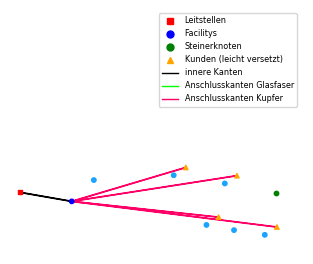
\includegraphics[width=\textwidth]{./Bilder/P2PGK_Naunyn_demand1_duration0}
	\end{minipage}
	\begin{minipage}[b]{0.4\textwidth}
		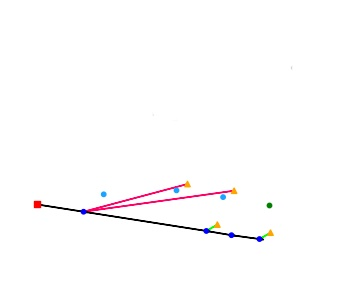
\includegraphics[width=\textwidth]{./Bilder/P2PGK_Naunyn_demand1_5_duration0}
	\end{minipage}
	\begin{minipage}[b]{0.4\textwidth}
		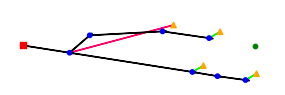
\includegraphics[width=\textwidth]{./Bilder/P2PGK_Naunyn_demand3_5_duration0}
	\end{minipage}
	\begin{minipage}[b]{0.4\textwidth}
		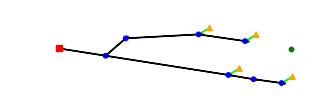
\includegraphics[width=\textwidth]{./Bilder/P2PGK_Naunyn_demand6_5_duration0}
	\end{minipage}
	\caption{Lösung des P2PGK mit verschiedenen Bedarfsfaktoren $d$ auf der Instanz Naunyn. Links oben: $d=1$, rechts oben: $d=1,5$, links unten $d=3,5$, rechts unten: $d=6,5$}
	\label{P2PGK_Naunyn_Bedarf}
\end{figure}

Die gleiche Analyse für Berlin und Vehlefanz fassen wir nun in den Tabellen \eqref{P2PGK_Berlin_Bedarf} und \eqref{P2PGK_Vehlefanz_Bedarf} (siehe Anhang) zusammen.
Dabei steht $A_G$ für die Anzahl der Kunden, die mit Glasfaser angeschlossen werden.
In Berlin gibt es insgesamt 39 Kunden und in Vehlefanz 238 Kunden.
In Tabelle \eqref{P2PGK_Berlin_Bedarf} erkennen wir, dass  bei einem Bedarfsfaktor $d$ von nur $1,5$ schon 10 Kunden mit Glasfaser angeschlossen werden und die Anzahl stetig steigt.
Bei einem Wert $d=5$ werden schon 33 von 39 Kunden mit Glasfaser angeschlossen.
Bei der Instanz Vehlefanz hingegen werden bei $d=5$ erst 57 von 238 Kunden mit Glasfaser angeschlossen. 
Ingesamt steigt die Anzahl der mit Glasfaser angeschlossenen Kunden deutlich langsamer als bei der Instanz Berlin.
Für jede Instanz und jeden Faktor $d$ ist die optimale Leitstelle, die gleiche.

Nun erweitern wir das P2PGK Problem, indem wir zusätzlich noch den Profit für den Anschluss eines Kunden betrachten.
Der monatliche Profit für den Anschluss eines Kunden $k \in K$ beträgt für Glasfaser $p_1(k)$ und für Kupfer $p_2(k)$, im folgenden betrachten wir dies als Profitfunktion $p:K \times \{1,2\} \rightarrow \Q_{ \geq 0 },(k,i) \mapsto p_i(k)$.
Dazu führen wir eine Variable $t$ für die Anzahl der betrachteten Monate ein.
Für $t=0$ entspricht das Problem dem P2PGK wie im Abschnitt zuvor.

Um diese Erweiterung unseres P2PGK Problems zu lösen, übergeben wir dem Algorithmus \ref{alg1} hierbei noch zusätzlich $t$ und $p$ und passen die Kostenfunktion \(c'\) \eqref{first_c_prime} wie folgt an.
\begin{align*}
c': A'' \rightarrow \Q, ij \mapsto \left\{\begin{array}{cl} 
c_{\text{dij}}(lj), & \text{falls } ij = lj \in D \text{ und } j \in F_1\\ 
c_{\text{dij}}(lj)+c(j), & \text{falls } ij = lj \in D \text{ und } j \in F_2\\ 
c(ij) + c(i) - t \cdot p_1(j), & \text{falls } ij \in A_1\\ 
c(ij) - t \cdot p_2(j), & \text{falls } ij \in A_2\\ 
\end{array}
\right.
\end{align*}
Außerdem erweitern wir das Steinerbaum Modell um die Bedingung 
\begin{align*}
	x_{ij} \leq \displaystyle\sum_{j \in K} y_{ij}^t \quad \forall ij \in A \text{ mit } c'(ij) \leq 0.
\end{align*}
Diese Nebenbedingung ist notwendig, da sonst alle Kanten $ij$ mit negativen Kosten ausgewählt werden.
Die Nebenbedingung verhindert dies, da nun nur die Kanten ausgew\"ahlt werden können, welche auch wirklich in dem Fluss vorkommen.
Es ist leicht zu sehen, dass der Algorithmus \ref{alg1} jetzt auch hierfür die optimale Lösung ausgibt. 

\textbf{Auswertung:}
Zuerst stellen wir fest, dass in unseren Instanzen der Profit einen Kunden $k \in K$ mit Glasfaser anzuschließen oft nur 4/3 des Profits $p_2(k)$ entspricht. 
Wir betrachten die Veränderung der Ergebnisse in 10-Jahres Schritten.
Für die Instanz Berlin und $t=0$ haben wir Kosten von 524.392 und es werden 3 Kunden mit Glasfaser angeschlossen.
Nach 10 Jahren sind die Kosten auf 366.112 gesunken bei gleichbleibender Anzahl von Kunden mit Glasfaseranschluss.
Erst bei einem Planungshorizont von 40 Jahren wird ein weiterer Kunde mit Glasfaser angeschlossen.
Da 40 Jahre \"ublicherweise ein zu großer Planungshorizont f\"ur ein Telekommunikationsunternehmen ist, ist es bei der Instanz Berlin nicht sinnvoll den Profit mit in die Planung einzubeziehen.
Bei den Instanzen Naunyn und Vehlefanz spielt der Profit sogar bei der Betrachtung eines Zeitraums von 40 Jahren keine Rolle f\"ur das optimale Netzwerk, denn selbst dann werden in den jeweiligen optimalen L\"osungen keine Kunden \"uber Glasfaser angeschlossen, siehe Tabelle \eqref{P2PGKProfitN} und \eqref{P2PGKProfitV}.
Dies liegt m\"oglicherweise daran, dass der Profitunterschied der verschiedenen Anschlusstechnologien in unseren Instanzen gering ist. Außerdem  bleibt die kostenminimale Leitstelle für jede Periode $t$ dieselbe.
Daher ist es f\"ur das Telekommunikationsunternehmen ratsam, die Netzwerke aufzubauen, die sich ohne die Ber\"ucksichtigung des Profits ergeben.

Zusammengefasst ist f\"ur die gegebenen Instanzen beim P2P Problem die Ber\"ucksichtigung einer steigenden Nachfrage an Bandbreite der Kunden wichtiger als die Betrachtung der verschiedenen Profite bei verschiedenen Anschlusstechnologien.

\section{Point-to-multipoint}
In diesem Kapitel behandeln wir die Point-to-multipoint Problemstellung.  Dabei betrachten wir erst den Fall, dass jeder Kunde durch eine Glasfaserkante angeschlossen werden muss. In dem darauffolgenden Abschnitt k\"onnen Kunden sowohl mit Glasfaser- als auch mit Kupferkabeln an das Netzwerk angeschlossen werden. Im letzten Abschnitt erweitern wir das P2MP mit Glasfaser und Kupfer Problem, indem wir auch monatliche Profite f\"ur den Anschluss eines Kunden mit einberechnen und indem wir unterschiedliche Nachfrage an Bandbreite in unser Modell einbeziehen. Außerdem betrachten wir die Möglichkeit verschiedene Arten Splitter zu installieren.

 
\subsection{Point-to-multipoint mit Glasfaser}
\label{section_p2mpg} 
 
Beim P2MP mit Glasfaser (P2MPG) Problem wollen wir jeden Kunden \"uber einen Glasfaseranschluss in das Netzwerk einbinden und dabei die entstehenden Kosten minimieren.
Anders als beim P2PG braucht nicht jeder Kunde eine eigene Leitung (bis auf die letzte Meile), sondern es k\"onnen auch Kabel durch einen Splitter in mehrere Kabel aufgeteilt werden.
Also m\"ussen wir bei diesem Problem wieder zuerst eine Leitstelle aus $L$ ausw\"ahlen und dann jeden Kunden an eine Facility anbinden, welche durch eine Glasfaserleitung an diese Leitstelle angebunden ist.
Falls nun ein Splitter in einen Knoten installiert wird und ein Glasfaserkabel in diesen Knoten ankommt, dann kann das eingehende Kabel in bis zu $a$ viele ausgehende Glasfaserkabel aufgeteilt werden, wobei wir in diesem Projekt f\"ur $a$ die Werte 4 und 16 betrachten.
In diesem Fall d\"urfen auch weitere Glasfaserkabel durch solch einen Knoten hindurchlaufen, die aber nicht ebenfalls aufgeteilt werden d\"urfen.

Dieses Problem lösen wir, indem wir das folgende Modell \ref{model_p2mpf} für jede Leitstelle $l \in L $ mit Gurobi \cite{gurobi} lösen und dann eine kostenminimale L\"osung davon ausw\"ahlen.
Sei dazu $A:= (I \backslash I_L) \cup A_1$, wobei $I_L$ die Menge der ausgehenden Kanten aus den nicht ausgewählten Leitstellen ist.
Dabei f\"ugen wir die inneren Kanten, die nicht von der Leitstelle \(l\) ausgehen, wieder als gerichtete Kanten in beide Richtungen mit identischen Kosten hinzu.
Die Entscheidungsvariable $y_{ij}^t \in \{0,1\}\; \forall ij \in A, t \in K$ modelliert einen Fluss von der Leitstelle $l$ zu dem Kunden $t$ für jeden Kunden.
Hier bedeutet $y_{ij}^t=1$, dass der Fluss von $l$ nach $t$ über die Kante $ij \in A$ fließt.
Die Variable $x_{ij} \in \Z_{\geq 0} \; \forall ij \in A $ gibt an, wie häufig die Kante \(ij\) in dem Netzwerk auftritt, also wie häufig wir diese Kante kaufen müssen.
Außerdem f\"uhren wir die binäre Entscheidungsvariable $s_i \in \{0,1\}$ für $i \in S \cup F$ ein.
Diese gibt an, ob in dem Knoten $i$ ein Splitter installiert wird ($s_i=1$) oder nicht ($s_i=0$).
Eine Splitterinstallation verursacht unabh\"angig von dem Knoten, in dem dieser installiert wird, Kosten \(c_s\) in H\"ohe der halben durchschnittlichen Kosten einer inneren Kante.
In diesem Modell entstehen also neben den Kosten f\"ur die Errichtung der Leitstelle weitere Kosten f\"ur die Installation eines Splitters und das Verlegen der Glasfaserkanten.
Daf\"ur ver\"andern wir die Kostenfunktion \eqref{Kostenfunktion} indem wir die Kosten für den Glasfaseranschluss eines Facility Knoten auf die Kantenkosten der jeweiligen Anschlusskante für den Glasfaseranschluss addieren.

\begin{align}
\label{KostenfunktionP2MP}
c': A \rightarrow \Q_{ \geq 0}, ij  \mapsto \left\{\begin{array}{cl} 
c(ij), & \text{falls } ij \in I\backslash I_L\\ 
c(ij)+c(i), & \text{falls } ij \in A_1\\ 
\end{array}
\right.
\end{align}
Also ergibt sich die folgende Minimierungsfunktion und insgesamt das folgende Modell.


 \bigskip
 $\min \displaystyle\sum_{ij \in A} c'(ij) x_{ij} + \displaystyle\sum_{i \in F \cup S} c_s s_i $
 \begin{align}\label{model_p2mpf}
 \begin{array}{rcrcrcll}
 \textrm{s.t.}  
&& &\displaystyle\sum_{ji \in A} y_{ji}^t - \displaystyle\sum_{ij \in A} y_{ij}^t& = & \left\{\begin{array}{cl} 
 -1, & \text{falls } i=l\\ 
 1, & \text{falls } i=t\\ 
 0, & \text{sonst.}\\ 
 \end{array}
 \right. & \forall t \in K & (1) \\
 &&& y_{ij}^t & \leq & x_{ij} & \forall ij \in A, t\in K & (2)\\
 &&& s_i &\leq& \displaystyle\sum_{ji \in A} x_{ji}& \forall  i \in S \cup F& (3)\\ 
 &0&\geq&\displaystyle\sum_{ji \in A} x_{ji} - \displaystyle\sum_{ij \in A} x_{ij}&\geq& -(a-1)s_i & \forall i \in S \cup F& (4)\\
 &&& y_{ij}^t & \in & \{0,1 \}& \forall ij \in A, t \in K & (5)\\
 &&& x_{ij} & \in & \Z _{\geq 0}& \forall ij \in A & (6)\\
 &&& s_i & \in & \{ 0,1 \} & \forall i \in S \cup F & (7) \\
 \end{array}
 \end{align}
Die Nebenbedingung (1) modelliert wie im Steinerbaum Problem mit Flussbedingung einen Fluss für jeden Kunden $t \in K$ von der Leitstelle $l$ zu dem Kunden.
Dabei gibt die Formel $\displaystyle\sum_{ji \in A} y_{ji}^t - \displaystyle\sum_{ij \in A} y_{ij}^t$ die Flusserhaltung an.
Falls diese Formel gleich -1 eins ist, geht also ein Fluss aus dem Knoten heraus, da keine Kante in die Leitstelle eingeht.
Das gleiche gilt für die Kunden, diese haben nur eingehende Kanten und somit gilt, falls die Formel gleich 1 ist, dass genau eine Flusskante in den Kundenknoten geht.
Ferner k\"onnen wir dem Programm noch die Information \"ubergeben, dass \(y_{ij}^t = 0\) ist, falls \(ij \in A_1 \cup A_2\) eine Anschlusskante ist und die Kante nicht zum Kunden \(t\) f\"uhrt, also \(j \neq t\) ist, da ein Fluss vom Kunden \(j\) nur in \(t\) enden soll, falls diese \"ubereinstimmen.
Die zweite Nebenbedingung stellt sicher, dass falls wir eine Kante in dem Fluss von $l$ nach $t$ benutzen, diese Kante auch in unserem Netzwerk gekauft wird.
Falls wir einen Splitter auf einem Knoten $i \in S \cup F$ benutzen, braucht dieser Splitter auch ein eingehendes Glasfaserkabel, dass dieser splitten kann.
Dies gewährleistet Bedingung (3).
Außerdem besitzen die $x_{ij}$ Variablen auch Flusserhaltung, modelliert in Bedingung (4).
Dies ist notwendig, da wir nur dann die Kabel aufteilen können, wenn wir auch einen Splitter installieren.
Falls wir keinen Splitter installieren, also $s_i=0$ ist, müssen genauso viele Kabel in den Knoten eingehen, wie auch wieder ausgehen, also $\displaystyle\sum_{ji \in A} x_{ji} - \displaystyle\sum_{ij \in A} x_{ij}=0$.
Falls wir einen Splitter installieren ($s_i=1$), kann eine eingehende Kante in bis zu $a$ Kanten aufgeteilt werden.
Deshalb darf die Summe der eingehenden Kanten maximal um \(a-1\) geringer sein als die Summe der ausgehenden Kanten.
Die Nebenbedingungen (5)-(7) wurden über dem Modell erklärt.
Das Model wird also für jede Leitstelle $l \in L$ gelöst und dann wird die Leitstelle $l \in L$ mit den minimalen Kosten ausgesucht. Die gesamt Kosten des Problems ergeben sich als Summe der Kosten des Models und der Kosten für den Aufbau der optimalen Leitstelle $l$. Dabei erhalten wir folgende Ergebnisse aus den Tabellen \ref{P2MPG_Tabelle_N_B} und \ref{P2MPG_Tabelle_V}.
  
Falls wir $a=1$ w\"ahlen l\"ost dieses Modell das P2PG Problem, denn dann ist die rechte Seite der Nebenbedingung (4) 0 und damit werden automatisch keine Splitter gekauft.
 
\textbf{Ergebnisse:}
 \begin{table}[h]
 	\centering
 	\begin{tabular}{c|c|c}
 		Instanz & Naunyn & Berlin \\	
 		\hline
 		 Kosten für $a=4$ & \(449.255,33\) & \(705.182,94\) \\
 		 Laufzeit auf PC1 & 0,046s & 2h 14m \\
 		 \hline
 		Kosten für $a=16$ & \(449.255,33\) & - \\
 		Laufzeit auf PC1 & 0,029s & - \\
 	\end{tabular}
 	\caption{Ergebnisse des P2MPG f\"ur Naunyn und Berlin}
 	\label{P2MPG_Tabelle_N_B}
 \end{table}
 
 Anmerkung zu Tabelle \eqref{P2MPG_Tabelle_N_B} Die Kosten f\"ur \(a=16\) bei der Instanz Berlin konnten wir lediglich zwischen den Werten \(702.663,48\) und \(705.182,94\) nach einer Laufzeit von etwa 3h 32m auf PC1 eingrenzen (Gap: \(0,36\) \%).
 
 \begin{table}[h]
 	\centering
 	\begin{tabular}{c|c|c|c|c}
 		Vehlefanz & untere Schranke & obere Schranke & Gap & Laufzeit auf PC1\\	
 		\hline
 		 Kosten für $a=4$ & \(1.528.315,57\) & \(1.537.043,86\) & 0,568\% & 10h 8m\\
 		 \hline
 		Kosten für $a=16$ & \(1.518.523,09\) & \(1.536.806,34\) & 1,18\% & 8h 20m \\
 	\end{tabular}
 	\caption{Ergebnisse des P2MPG f\"ur Vehlefanz}
 	\label{P2MPG_Tabelle_V}
 \end{table}
 
Auffallend ist die m\"oglicherweise noch sehr geringe, aber vielleicht auch gar nicht vorhandene Differenz der Kosten f\"ur die Werte von 4 und 16 von \(a\).
Bei der L\"osung f\"ur \(a=4\) bei Naunyn wird lediglich ein Splitter installiert und dieser teilt ein eingehendes Glasfaserkabel in zwei ausgehende auf, daher ver\"andert sich die optimale L\"osung auch nicht, wenn mehr ausgehende Kanten erlaubt sind.
Bei der Instanz Berlin bei \(a=4\) gibt es ebenfalls in einem Splitter maximal 3 ausgehende Glasfaserkanten.
Daher ist es auch hier nicht verwunderlich, dass die optimale L\"osung f\"ur \(a=16\) nicht oder nur sehr wenig von der von \(a=4\) abweicht.
Da wir nur eine obere Schranke der optimalen L\"osung f\"ur \(a=4\) bei Vehlefanz bekommen haben, in dieser aber bereits ebenfalls nur wenige Splitter 3 oder mehr ausgehende Glasfaserkanten besitzen, ist die maximale Differenz der Kosten f\"ur die Werte 4 und 16 von \(a\) in H\"ohe von etwas weniger als nur 30.000 naheliegend.
Die eben angef\"uhrten maximalen Anzahlen an Splittern erkennen wir auch an den Abbildungen \eqref{p2mpg_n_pic}, \eqref{p2mpg_b_pic} und \eqref{p2mpg_v_pic_ub}.
Insbesondere f\"allt auch der kaum vorhandene Unterschied der graphischen Darstellungen der oberen Schranken in der Instanz Vehlefanz f\"ur \(a=4\) \eqref{p2mpg_v_pic_ub} und \(a=16\) \eqref{p2mpg_v_sn16_pic_ub} auf.

Wir k\"onnten jetzt eine Analyse anf\"uhren, wie sich die Kosten des P2MPG ver\"andern w\"urden, falls nicht nur ein Splitter, sondern unendlich viele Splitter gleichzeitig in einen Knoten installiert werden d\"urften.
Da wir aber bereits oben gesehen haben, dass eine erlaubte Anzahl von 16 ausgehenden Kanten nichts oder nur sehr wenig am Ergebnis \"andert, ist diese Analyse unn\"otig, da sich das Ergebnis auch nicht von den obigen unterscheiden w\"urde.
Wenn bereits bei 12 weiteren kostenlos zusammenfassbaren Glasfaserkanten nichts am Netzwerk \"andert, w\"urden auch keine weiteren Splitter installiert werden, die sogar weitere Kosten verursachen w\"urden.
 
\subsection{Point-to-multipoint mit Glasfaser und Kupfer}

Nun betrachten wir auch wieder den Fall, dass Kunden sowohl \"uber Kupferkabel, als auch \"uber Glasfaserkabel angeschlossen werden k\"onnen.
Dabei kann in einem Facility Knoten von Typ 2 jedoch nur entweder ein DSLAM oder ein Splitter installiert werden.
Dieses Problem lösen wir mit einer Erweiterung des linearen Programms \ref{model_p2mpf} des P2MPG Problems.
Dazu erweitern wir den Graphen \(G = (V,A)\) und die Kostenfunktion \(c'\) \eqref{KostenfunktionP2MP} aus \ref{section_p2mpg} wie folgt.
Den Kanten des Graphen f\"ugen wir zus\"atzlich noch die Anschlusskanten von Typ 2 hinzu, also \(A := (I \backslash I_L ) \cup A_1 \cup A_2\).
Weiterhin erweitern wir die Kostenfunktion auch auf die Kanten aus \(A_2\).
\begin{align}
\label{KostenfunktionP2MPGK}
c': A \rightarrow \Q_{ \geq 0}, ij  \mapsto \left\{\begin{array}{cl} 
c(ij), & \text{falls } ij \in (I\backslash I_L) \cup A_2\\ 
c(ij)+c(i), & \text{falls } ij \in A_1\\ 
\end{array}
\right.
\end{align}
Wir l\"osen dieses Problem wieder, indem wir das folgende Modell \ref{model_p2mpgk} für jede Leitstelle $l \in L $ mit Gurobi \cite{gurobi} lösen und dann eine kostenminimale L\"osung davon ausw\"ahlen.

Die Entscheidungsvariablen $y_{ij}^t,x_{ij}$ und $s_i$ seien definiert wie in dem P2MPG Modell \ref{model_p2mpf} und f\"ur die Kanten aus \(A_2\) analog definiert.
Ebenfalls \"ubergeben wir dem Programm die Bedingung, dass \(y_{ij}^t = 0\) ist, falls \(ij \in A_1 \cup A_2\) eine Anschlusskante und \(j \neq t\) ist.
Wir fügen noch eine Entscheidungsvariable $m_i \in \{0,1\} \forall i \in F_2$ hinzu, die angibt, ob in einer Facility \(i \in F_2\) von Typ 2 ein DSLAM installiert ist (\(m_i = 1\)) oder nicht (\(m_i = 0\)).
Die Zielfunktion des Modells wird deswegen noch durch den Summanden $\displaystyle\sum_{i \in F_2} c(i) m_i$ erweitert.
Insgesamt ergibt sich das nachfolgende Modell.

  \bigskip
  $\min \displaystyle\sum_{ij \in A} c'(ij) x_{ij} + \displaystyle\sum_{i \in F \cup S} c_s s_i + \displaystyle\sum_{i \in F_2} c(i) m_i$
  \begin{align}\label{model_p2mpgk}
  \begin{array}{rcrcrcll}
  \textrm{s.t.}  
  && &\displaystyle\sum_{ji \in A} y_{ji}^t - \displaystyle\sum_{ij \in A} y_{ij}^t& = & \left\{\begin{array}{cl} 
  -1, & \text{falls } i=l\\ 
  1, & \text{falls } i=t\\ 
  0, & \text{sonst.}\\ 
  \end{array}
  \right. & \forall t \in K & (1) \\
  &&& y_{ij}^t & \leq & x_{ij} & \forall ij \in A, t\in K & (2)\\
    &&& s_i &\leq& \displaystyle\sum_{ji \in A} x_{ji}& \forall  i \in S \cup F & (3)\\ 
  &0&\geq&\displaystyle\sum_{ji \in A} x_{ji} - \displaystyle\sum_{ij \in A} x_{ij}&\geq& -(a-1)s_i & \forall i \in S \cup F_1& (4)\\
   &0&\geq&\displaystyle\sum_{ji \in A} x_{ji} -m_i - \displaystyle\sum_{ij \in I \cup A_1} x_{ij}&\geq& -(a-1)s_i & \forall i \in F_2& (4')\\
   &&&s_i+m_i & \leq & 1 & \forall i \in F_2 & (8)\\
   &&&x_{ij}& \leq & m_i & \forall i \in F_2, ij \in A_2 & (9) \\
    &&& y_{ij}^t & \in & \{0,1 \}& \forall ij \in A, t \in K & (5)\\
    &&& x_{ij} & \in & \Z_{\geq 0} & \forall ij \in A & (6)\\
    &&& s_i & \in & \{ 0,1 \} & \forall i \in S \cup F & (7) \\
    &&& m_i & \in & \{ 0,1 \} & \forall i \in F_2 & (10) \\
  \end{array}
  \end{align}
  
Die Nebenbedingung (4) aus dem P2MPG Modell bleibt für die Knoten aus $S \cup F$ unver\"andert.
In den Knoten aus $F_2$ können wir nun auch einen Multiplexer installieren.
Dies müssen wir auch bei der Flusserhaltung der $x_{ij}$ beachten.
Die Nebenbedingung \((4')\) modelliert den Fluss der $x_{ij}$ für die Knoten $i \in F_2$.
Falls ein Splitter installiert wird, kann kein Multiplexer installiert werden und die Bedingung entspricht der Bedingung (4) aus dem P2MPG Modell.
Falls ein Multiplexer $i \in F_2$ installiert wird ($m_i=1$), geht ein Glasfaserkabel in den Multiplexer ein und es k\"onnen unendlich viele Kupferkabel, also Anschlusskanten von Typ 2, hinaus gehen.
Jedoch muss die Flusserhaltung f\"ur die inneren Kanten und die Anschlusskanten von Typ 1 erhalten bleiben.
Dies modelliert die Gleichung $\displaystyle\sum_{ji \in A} x_{ji} -1 - \displaystyle\sum_{ij \in I \cup A_1} x_{ij}=0$.
In jedem Knoten aus $F_2$ kann entweder ein Multiplexer oder ein Splitter installiert werden, nicht beides gleichzeitig.
Dies wird durch die Nebenbedingung (8) sichergestelllt.
Außerdem d\"urfen nur Kupferkabel aus einer Facility gehen, falls auch ein Multiplexer installiert ist, was in Nebenbedingung (9) modelliert wird.
Die Entscheidungsvariablen (5)-(7) und (10) wurden schon \"uber dem Modell erkl\"art.   

Das Model wird also für jede Leitstelle $l \in L$ gelöst und dann wird die Leitstelle $l \in L$ mit den minimalen Kosten ausgesucht. Die gesamt Kosten des Problems ergeben sich als Summe der Kosten des Models und der Kosten für den Aufbau der optimalen Leitstelle $l$. Dabei erhalten wir folgende Ergebnisse.

 \begin{table}[h]
	\centering
	\begin{tabular}{c|c|c|c}
		Instanz & Naunyn & Berlin & Vehlefanz \\	
		\hline
		Kosten für $a=4$ & 397.662,0 & 474.909,28 & 587.503,28 \\
		Laufzeit auf PC1 & 0,03s & 7m 13s & 14m 55s \\
		\hline
		Kosten für $a=16$ & 397.662,0 & 474.909,28 & -\\
		Laufzeit auf PC1 & 0,03s & 27m 12s & - \\
	\end{tabular}
	\caption{Ergebnisse des P2MPGK}
	\label{P2MPGK}
\end{table}

Bei den optimalen Werten von den P2MPG und P2MPGK Problemen ist die prozentuale Ver\"anderung deutlich geringer als zwischen den P2PG und P2PGK Problemen.
Hier betr\"agt diese nur noch \(88,51\) \% bei Naunyn und \(67,35\) \% bei Berlin.

Bei diesen Ergebnissen ist wieder auff\"allig, dass f\"ur die Instanzen Naunyn und Berlin sich die gleichen Ergebnisse bei den Werten 4 und 16 f\"ur \(a\) ergeben, jedoch mit einer fast vierfach so langen Laufzeit f\"ur die Instanz Berlin.
Wir haben uns auch hier bereits die L\"osung des P2MPGK f\"ur \(a=4\) bei Vehlefanz angeschaut und bemerkt, dass die Anzahl der aus einem Splitter ausgehenden Glasfaserkanten maximal 2 betr\"agt.
Daher haben wir die Kosten f\"ur \(a = 16\) gar nicht mehr berechnet mit der gleichen \"Uberlegung wie aus Abschnitt \ref{section_p2mpg}.
Ebenso k\"onnen wir mit der gleichen Begr\"undung wie in \ref{section_p2mpg} sagen, dass die Betrachung der M\"oglichkeit unendlich viele Splitter in einem Knoten installieren zu k\"onnen, nicht sinnvoll ist. Es ist sehr wahrscheinlich, dass sich durch Installation unendlich vieler Splitter in einem Knoten die Kosten nicht mehr ändern.
Das optimale Netzwerk für $a=4$ der verschiedenen Instanzen ist in den Abbildungen \eqref{p2mpgk_n_pic_sn4}, \eqref{p2mpgk_b_pic_sn4} und \eqref{p2mpgk_v_pic_sn4} zu sehen. Die Abbildungen \eqref{p2mpgk_n_pic_sn16}, \eqref{p2mpgk_b_pic_sn16} veranschaulichen das optimale Netzwerk für die verschiedenen Instanzen für $a=16$.
   
 \subsection{Erweiterung des P2MP mit Glasfaser und Kupfer}
Wie beim P2PGK Problem in Abschnitt \ref{Erweiterung des P2PGK} kann man auch hier mit verschiedenen monatlichen Profiten f\"ur jeden Kunden rechnen oder einen steigenden Bedarf an Bandbreite betrachten. Diese Probleme betrachten wir nur für den Parameter $a=4$.
Außerdem betrachten wir die Möglichkeit zwei Splitter mit unterschiedlichen Kosten und mit einer anderen Splitterzahl $a$ zu installieren.
 
Um den voraussichtlich steigenden Bedarf an Bandbreite eines Kunden zu modellieren, haben wir genau wie in Abschnitt \ref{Erweiterung des P2PGK} den angegebenen Bedarf mit verschiedenen Werten $d$ multipliziert und dann die Kanten gel\"oscht, die diesen Bedarf der Kunden nicht decken (siehe Abschnitt \ref{preprocess}), um dann mit diesem neuen Graphen das P2MPGK Problem zu l\"osen.
 
 \textbf{Auswertung:} Betrachten wir die Tabellen mit den Ergebnissen f\"ur die Instanzen Naunyn \eqref{P2MPGKBedarfN}, Berlin \eqref{P2MPGKBedarfB} und Vehlefanz \eqref{P2MPGKBedarfV}, so ist zu erkennen, dass die Anzahl der mit Glasfaser angeschlossenen Kunden bei Naunyn und Berlin sehr schnell und bei Vehlefanz nur langsam steigt.
 F\"ur die Instanz Berlin haben wir bereits bei einem Bedarfsfaktor von \(d=2\) \"uber 2/3 der Kunden mit Glasfaser angeschlossen.
 In dieser Instanz ist es f\"ur das Telekommunikationsunternehmen sinnvoll den Bedarfsfaktor zu ber\"ucksichtigen.
Bei Vehlefanz hingegen haben wir erst ab einem Bedarfsfaktor von \(3,5\) einen gr\"oßeren Sprung bei der Anzahl der mit Glasfaser angeschlossenen Kunden von 14 auf 40.
Im Verh\"altnis zur Gesamtzahl der Kunden von 238 ist dieser Anteil dennoch sehr gering. 
Nat\"urlich ist die Aktualit\"at der erhobenen Daten zu ber\"ucksichtigen, aber bei einem heutigen Stand der Technik und des Bedarfs ist ein Anstieg der Nachfrage auf das dreifache oder mehr in den n\"achsten Jahren wohl nicht zu erwarten, daher lohnt sich f\"ur das Telekommunikationsunternehmen die Betrachtung der Nachfrage f\"ur die Instanz Vehlefanz kaum. 
Diese Analyse ergibt dasselbe wie für das P2PGK Problem mit Bedarfsfaktor $d$, da dieselben Kunden mit Glasfaser angeschlossen werden müssen.
Zum Beispiel werden bei der Instanz Vehlefanz bei $d=3,5$ sowohl bei P2PGK als auch bei P2MPGK 40 Kunden \"uber Glasfaser angeschlossen.
Die optimale Leitstelle bleibt bei diesen Betrachtungen für jeden Faktor $d$ unver\"andert. 
  
Nun erweitern wir das P2MPGK Problem, indem wir zusätzlich noch den Profit für den Anschluss eines Kunden betrachten.
Auch hier gehen wir genauso vor wie in Abschnitt \ref{Erweiterung des P2PGK}.
Wieder gibt die Variable $t$ den Planungshorizont in Monaten an.
Wir \"ubergeben unserem Modell also noch die Variable $t$ und die Profitfunktion $p$.
Außerdem \"andern wir die Kostenfunktion \(c'\) \eqref{KostenfunktionP2MP}  zu folgender Funktion:
\begin{align*}
  c'': A  \rightarrow \Q,  ij  \mapsto \left\{\begin{array}{cl} 
 c'(ij), & \text{falls } ij \in I\backslash I_L \\ 
  c'(ij) -t  \cdot p_1(j), & \text{falls } ij \in A_1 \\ 
    c'(ij) -t \cdot p_2(j), & \text{falls } ij \in  A_2 \\ 
\end{array}  \right.
\end{align*}
Außerdem erweitern wir auch das P2MPGK Modell durch die Nebenbedingung 
\begin{align*}
 x_{ij} \leq \displaystyle\sum_{t \in K} y_{ij}^t \quad \forall ij \in A \text{ mit } c''(ij) \leq 0.
\end{align*}

Diese Nebenbedingung ist ebenfalls wie bei der Erweiterung des P2P Problems notwendig, da sonst alle Kanten $ij$ mit negativen Kosten ausgewählt werden und die Nebenbedingung dies verhindert, da nun nur die Kanten ausgew\"ahlt werden können, welche auch wirklich in dem Fluss vorkommen.
 
 \textbf{Auswertung:} Bei den Ergebnissen des P2MPGK Problems mit Ber\"ucksichtigung der verschiedenen Profite f\"ur die drei Instanzen \eqref{P2MPGKProfitN}, \eqref{P2MPGKProfitB} und \eqref{P2MPGKProfitV} lassen sich einige Gemeinsamkeiten erkennen.
 Bei den Instanzen Naunyn und Berlin werden erst ab einer Betrachtung von 40 Jahren mindestens die H\"alfte der Gesamtzahl der Kunden (4 bzw. 39) mit Glasfaserkanten angeschlossen.
 Bei Naunyn wird sogar bei einer Betrachtung von 30 Jahren noch kein Kunde mit Glasfaser angeschlossen.
 Im Gegensatz zum P2PGK Problem (bei diesem wurde erst nach 40 Jahren ein Kunde mehr mit Glasfaser angeschlossen) werden bei Berlin bereits nach 10 Jahren schon 5 Kunden mit Glasfaser angeschlossen. Die Anzahl steigt dennoch recht langsam. Da ein Zeitraum von 30 oder gar 40 Jahren den \"ublichen Planungshorizont eines Telekommunikationsunternehmens \"ubersteigt, sollte das Unternehmen diese Profite der verschiedenen Anschlusstechnologien nicht ber\"ucksichtigen.  Das heißt, es sollten eventuell nun 7 Kunden anstatt 3 mit Glasfaser angeschlossen werden, aber nicht 24, wie nach 40 Jahren.  Die Analyse der Ergebnisse für Vehlefanz aus Tabelle \ref{P2MPGKProfitV} ergibt dasselbe Ergebnis.
 Erwähnenswert ist noch, dass für jede Instanz die Leitstelle für jede Periode $t$ dieselbe bleibt.

 
Betrachten wir nun die Möglichkeit, dass zwei unterschiedliche Splitterarten installiert werden können.
Dazu seien die Kosten des ersten Splitters $c_s$ und es sei $a$ die Anzahl der ausgehenden Kanten des Splitters.
Die Kosten des zweiten Splitters seien $c_{s'}$ und $a'$ sei die Anzahl der ausgehenden Kanten dieses Splitters.
Dazu erweitern wir beide Modelle des P2MP Problems \ref{model_p2mpf} und \ref{model_p2mpgk} durch eine zusätzliche Variable $s'_i \in \{0,1\} \forall i \in S\cup F$.
Diese gibt an, ob der zweite Splitter in Knoten i installiert wird ($s'_i=1$) oder nicht ($s'_i=0$).
Zu der Zielfunktion addieren wir noch den Summanden $\displaystyle\sum_{i \in F \cup S} c_{s'} s'_i$.
Außerdem ändern wir die Nebenbedingung (4) bzw. $(4')$ und fügen die nachfolgenden zusätzlichen Nebenbedingungen hinzu.

  \begin{align*}
  \begin{array}{rcrcrcll}
  &0&\geq&\displaystyle\sum_{ji \in A} x_{ji} - \displaystyle\sum_{ij \in A} x_{ij}&\geq& -(a-1)s_i -(a'-1)s'_i & \forall i \in S \cup F_1& (4)\\
  &0&\geq&\displaystyle\sum_{ji \in A} x_{ji} (-m_i) - \displaystyle\sum_{ij \in I \cup A_1} x_{ij}&\geq& -(a-1)s_i -(a'-1)s'_i & \forall i \in F_2& (4')\\
    &&&s_i+s'_i & \leq &1 & \forall i \in S \cup F_1,ij\in A_2& (8')\\
  &&&s_i+s'_i(+m_i) & \leq &1 & \forall i \in F_2,ij\in A_2 &   (8'')\\
  &&& s'_i & \in & \{ 0,1 \} & \forall i \in S \cup F & (11) \\
  \end{array}
  \end{align*}

Dabei lassen wir das \(m_i\) in den Nebenbedingungen (\(4'\)) und (\(8''\)) f\"ur das P2MPG Modell \eqref{model_p2mpf} weg, da in diesem Fall keine Multiplexer installiert werden k\"onnen.
 
 \section{Zusammenfassung}
In diesem Kapitel veranschaulichen wir unsere gesamten Ergebnisse auf allen drei Instanzen der verschiedenen Probleme noch einmal graphisch. Dazu sind die Ergebnisse der Probleme P2P mit Glasfaser, P2P mit Kupfer und Glasfaser mit Bedarfsfaktoren $d=1, d=1,5, d=3$, P2MP mit Glasfaser und P2MP mit Kupfer und Glasfaser mit Bedarfsfaktoren $d=1, d=1,5, d=3$ der Größe nach sortiert in einem Balkendiagramm dargestellt. Wir betrachten die P2MP Probleme nur für $a=4$.

  \begin{figure}[!htbp]
  	\centering
 	\begin{tikzpicture}
 	\begin{axis}[
 	symbolic x coords={P2PGK1,P2MPGK1,P2MPGK1.5,P2MPGK3,P2PGK1.5,P2PGK3,P2MPG,P2PG},
 	x tick label style={rotate=45,anchor=east},
 	height=6cm, width=10cm,
 	bar width=0.4cm,
 	enlarge x limits=true,
 	ylabel=Kosten]
 	\addplot[ybar,fill=red] coordinates {
 		(P2PGK1,      397622)
 		(P2PGK1.5,   442842)
 		(P2PGK3,        442842)
 		(P2PG,        480722)};
 	\addplot[ybar,fill=blue] coordinates {
 		(P2MPG,   449255)
 		(P2MPGK1,      397622)
 		(P2MPGK1.5,   427533)
 		(P2MPGK3,   427533)};
 	\end{axis}
 	\end{tikzpicture}
 	\caption{\"Ubersicht der Ergebnisse der Instanz Naunyn}
 \end{figure}
 
 Da es in der Instanz Naunyn nur 4 Kunden gibt, ist diese Instanz zu klein und bei verschiedenen Problemen entstehen die gleichen Lösungen. Zum Beispiel sind die Lösungen des P2PGK und des P2MPGK identisch, siehe Abbildungen \eqref{p2pgk_n_pic} und \eqref{p2mpgk_n_pic_sn4}.
 
 \begin{figure}[!htbp]
 	\centering
 	\begin{tikzpicture}
 	
 	\begin{axis}[
 	symbolic x coords={P2MPGK1,P2PGK1,P2MPGK1.5,P2MPGK3,P2MPG,P2PGK1.5,P2PGK3,P2PG },
 	x tick label style={rotate=45,anchor=east},
 	height=6cm, width=10cm,
 	bar width=0.4cm,
 	enlarge x limits=true,
 	ylabel=Kosten]
 	\addplot[ybar,fill=red] coordinates {
 		(P2PGK1,      524392)
 		(P2PGK1.5,   709412)
 		(P2PGK3,        1142322)
 		(P2PG,        1388562)};
 	\addplot[ybar,fill=blue] coordinates {
 		(P2MPG,   705182)
 		(P2MPGK1,      474909)
 		(P2MPGK1.5,   543177)
 		(P2MPGK3,    653629)};
 	\end{axis}
 	\end{tikzpicture}
 	\caption{\"Ubersicht der Ergebnisse der Instanz Berlin}
 \end{figure}
 
 Bei der Instanz Berlin ist sehr auffällig, dass die Lösung des P2PGK für $d=1,5$ und $d=3$ teurer sind als die Lösung des P2MP, wobei alle Kunden mit Glasfaser angeschlossen werden. Das heißt, in dieser Instanz ist es sehr teuer, Kunden nachträglich mit Glasfaser anzuschließen, da der Kostenunterschied zwischen P2PGK mit $d=1$ und P2PGK mit $d=3$ nur an der erhöhten Anzahl von Glasfaserkunden liegt. 
 
 
  \begin{figure}[!htbp]
  	\centering
 	\begin{tikzpicture}
 	\begin{axis}[
 	symbolic x coords={P2MPGK1, P2MPGK1.5,P2PGK1,P2PGK1.5,P2MPGK3,P2PGK3,P2MPG,P2PG},
 	x tick label style={rotate=45,anchor=east},
 	height=6cm, width=10cm,
 	bar width=0.4cm,
 	enlarge x limits=true,
 	ylabel=Kosten]
 	\addplot[ybar,fill=red] coordinates {
 		(P2PGK1,      647408)
 		(P2PGK1.5,  647608)
 		(P2PGK3,        1274782)
 		(P2PG,        7791258)};
 	\addplot[ybar,fill=blue] coordinates {
 		(P2MPG,   1537043)
 		(P2MPGK1,      587503)
 		(P2MPGK1.5,   587503)
 		(P2MPGK3,   677145)};
 	\end{axis}
 	\end{tikzpicture}
 	\caption{\"Ubersicht der Ergebnisse der Instanz Vehlefanz}
 \end{figure}
F\"ur unsere gr\"oßte Instanz Vehlefanz ist sehr auff\"allig, dass im Verhältnis die Kosten sowohl f\"ur das P2PGK mit Bedarfsfaktoren 1 und 1,5 als auch f\"ur das P2MPGK mit Bedarfsfaktoren 1, 1,5 und 3 nicht stark variiere.
Dahingegen weichen die Kosten f\"ur reinen Glasfaseranschluss deutlich nach oben ab.

Wir kommen zu unserem Fazit, dass das P2MPGK Problem auch mit Bedarfsfaktoren und Profiten h\"aufig kosteng\"unstigere L\"osungen liefert als das P2PGK Problem mit nur wenigen erh\"ohten Bedingungen.
Daher ist es deutlich kosteng\"unstiger f\"ur ein Telekommunikationsunternehmen, auf das P2MPGK Modell zur\"uckzugreifen.
Ist man hingegen an einer m\"oglichst schnell zu generierenden L\"osung interessiert, so lohnt sich eher das P2PGK Modell.
\newpage
\bibliographystyle{babplain-lf}
\renewcommand{\refname}{Literaturverzeichnis}
\bibliography{literatureProject1}
\newpage
\appendix
\section*{Abbildungsverzeichnis}

\begin{figure}[!htbp]
	\begin{center}
		\begin{minipage}{10.0cm}
			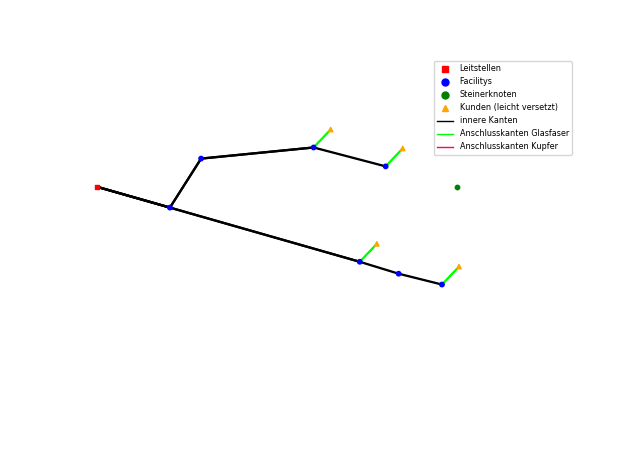
\includegraphics[width=1\textwidth]{./Bilder/P2PG_Naunyn}
			\caption{Lösung des P2PG Problems auf der Instanz Naunyn}
			\label{fig:p2pg n pic}
		\end{minipage}
	\end{center}
\end{figure}

\begin{figure}[!htbp]
\begin{center}
	\begin{minipage}{15.0cm}
		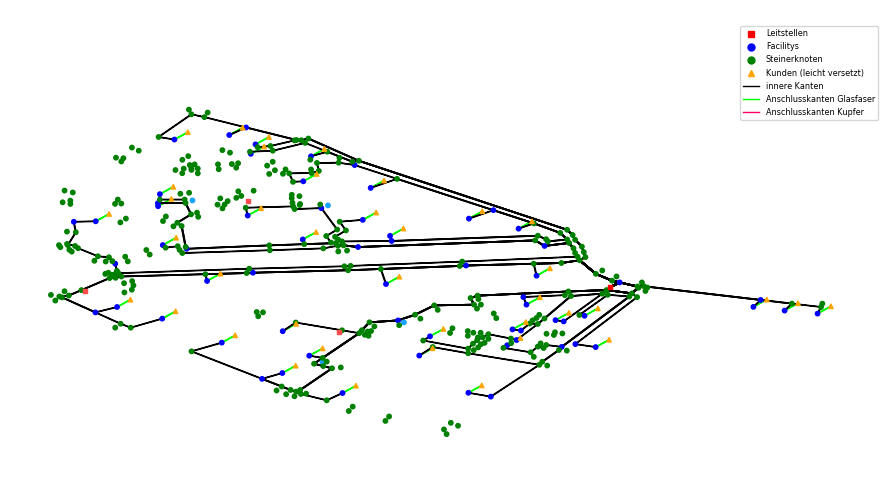
\includegraphics[width=1\textwidth]{./Bilder/P2PG_Berlin}
		\caption{Lösung des P2PG Problems auf der Instanz Berlin}
		\label{p2pg b pic}
	\end{minipage}
\end{center}
\end{figure}

\begin{figure}[!htbp]
\begin{center}
	\begin{minipage}{15.0cm}
		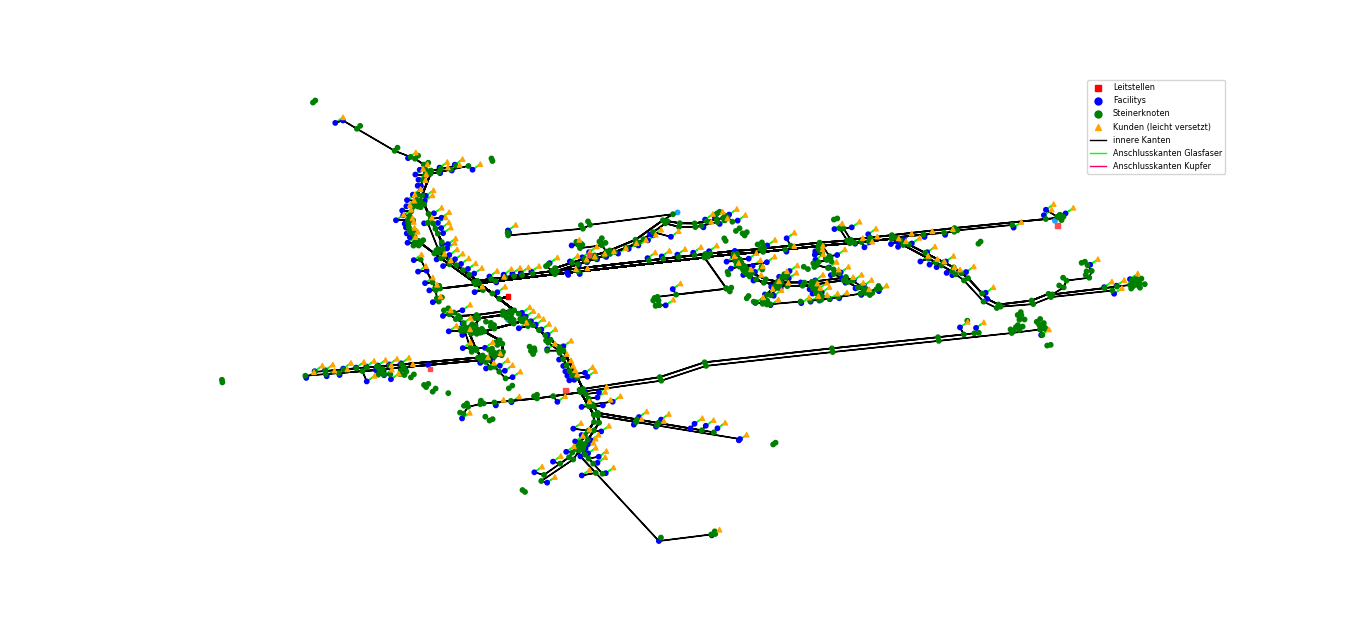
\includegraphics[width=1\textwidth]{./Bilder/P2PG_Vehlefanz}
		\caption{Lösung des P2PG Problems auf der Instanz Vehlefanz}
		\label{p2pg v pic}
	\end{minipage}
\end{center}
\end{figure}


\begin{figure}[!htbp]
	\begin{center}
		\begin{minipage}{8.0cm}
			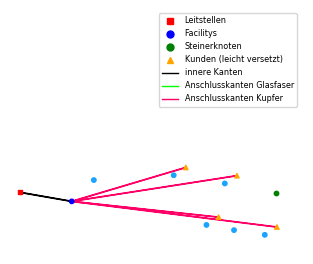
\includegraphics[width=1\textwidth]{./Bilder/P2PGK_Naunyn_demand1_duration0}
			\caption{Lösung des P2PGK Problems auf der Instanz Naunyn}
			\label{p2pgk_n_pic}
		\end{minipage}
	\end{center}
\end{figure}

\begin{figure}[!htbp]
	\begin{center}
		\begin{minipage}{15.0cm}
			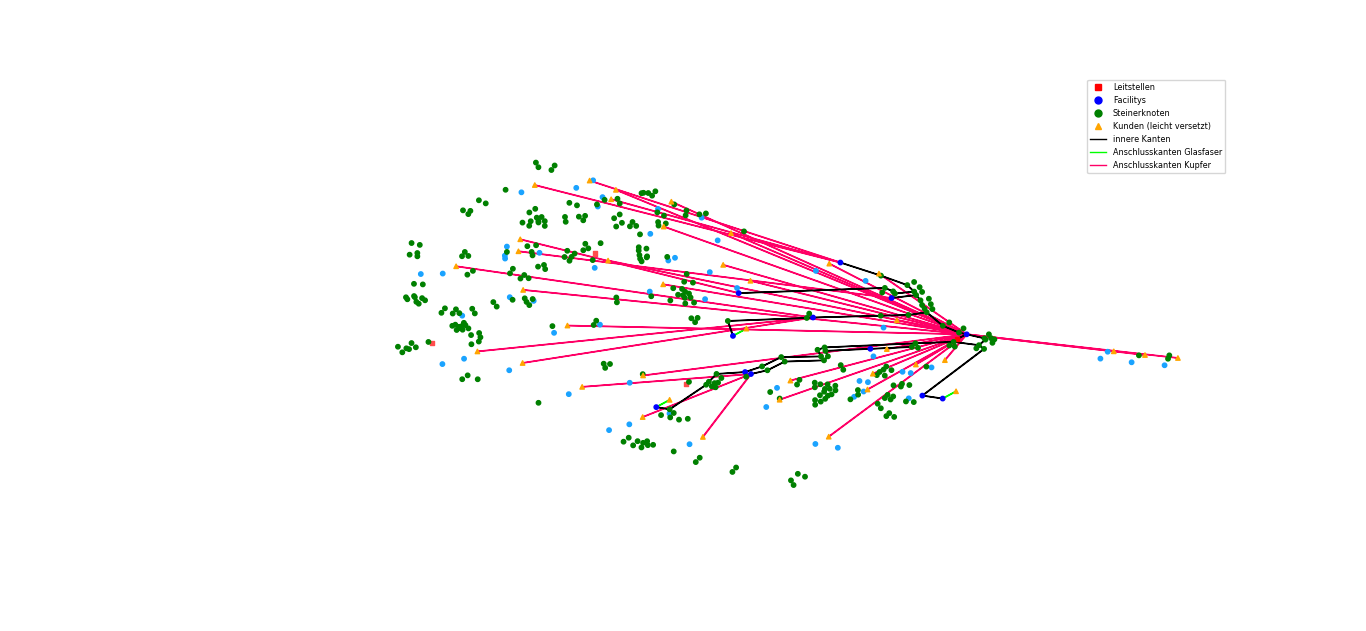
\includegraphics[width=1\textwidth]{./Bilder/P2PGK_Berlin_demand1_duration0}
			\caption{Lösung des P2PGK Problems auf der Instanz Berlin}
			\label{p2pgk_b_pic}
		\end{minipage}
	\end{center}
\end{figure}

\begin{figure}[!htbp]
	\begin{center}
		\begin{minipage}{15.0cm}
			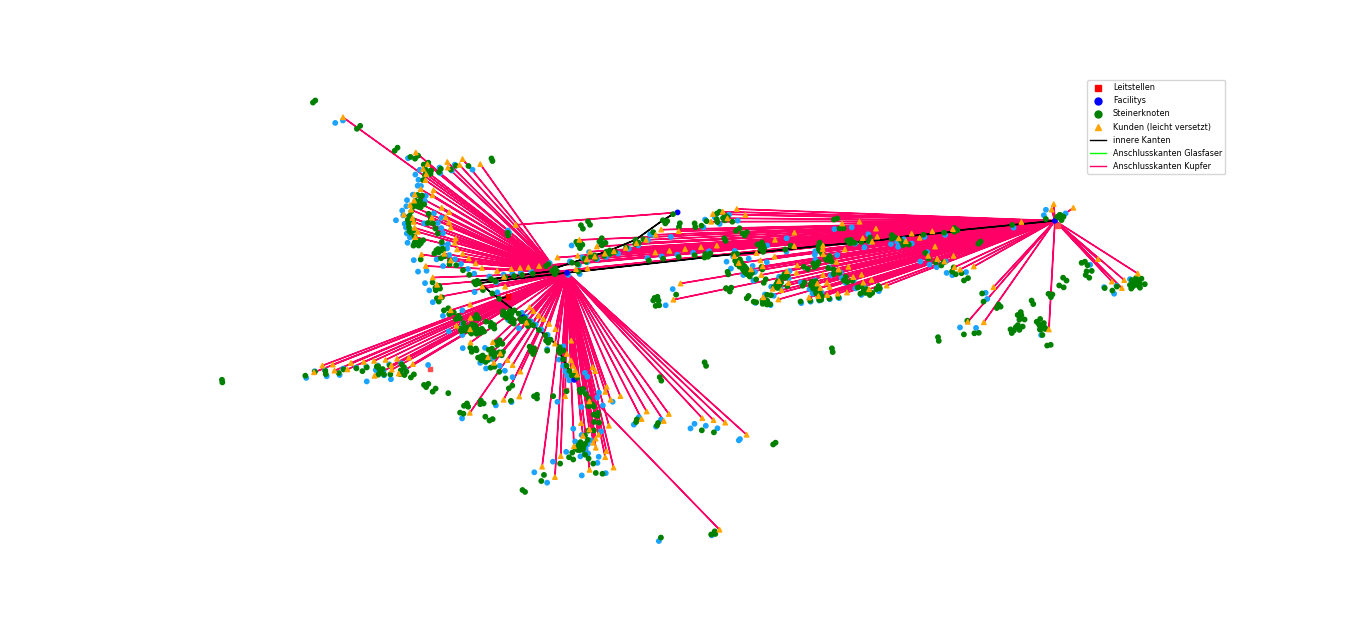
\includegraphics[width=1\textwidth]{./Bilder/P2PGK_Vehlefanz_demand1_duration0}
			\caption{Lösung des P2PGK Problems auf der Instanz Vehlefanz}
			\label{p2pgk_v_pic}
		\end{minipage}
	\end{center}
\end{figure}

\begin{figure}[!htbp]
	\begin{center}
		\begin{minipage}{8.0cm}
			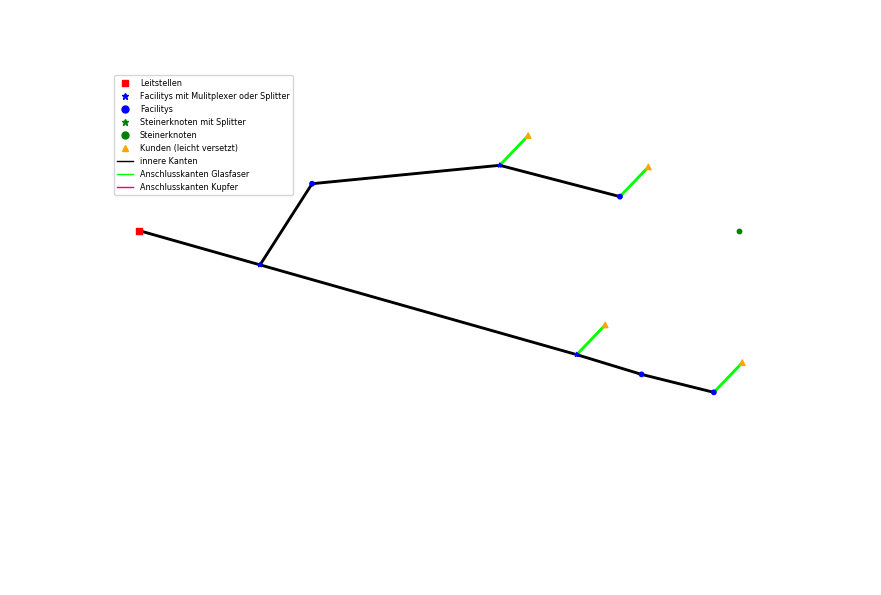
\includegraphics[width=1\textwidth]{./Bilder/P2MPG_Naunyn_demand1_duration0}
			\caption{Lösung des P2MPG Problems f\"ur \(a=4\) auf der Instanz Naunyn}
			\label{p2mpg_n_pic}
		\end{minipage}
	\end{center}
\end{figure}

\begin{figure}[!htbp]
	\begin{center}
		\begin{minipage}{15.0cm}
			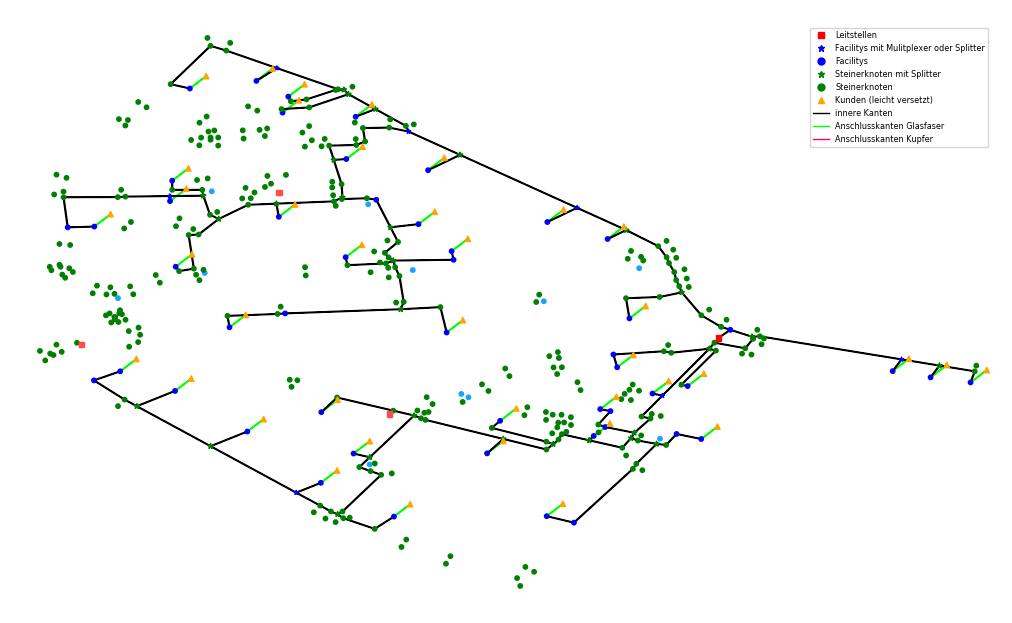
\includegraphics[width=1\textwidth]{./Bilder/P2MPG_Berlin_demand1_duration0}
			\caption{Lösung des P2MPG Problems f\"ur \(a=4\) auf der Instanz Berlin}
			\label{p2mpg_b_pic}
		\end{minipage}
	\end{center}
\end{figure}

\begin{figure}[!htbp]
	\begin{center}
		\begin{minipage}{15.0cm}
			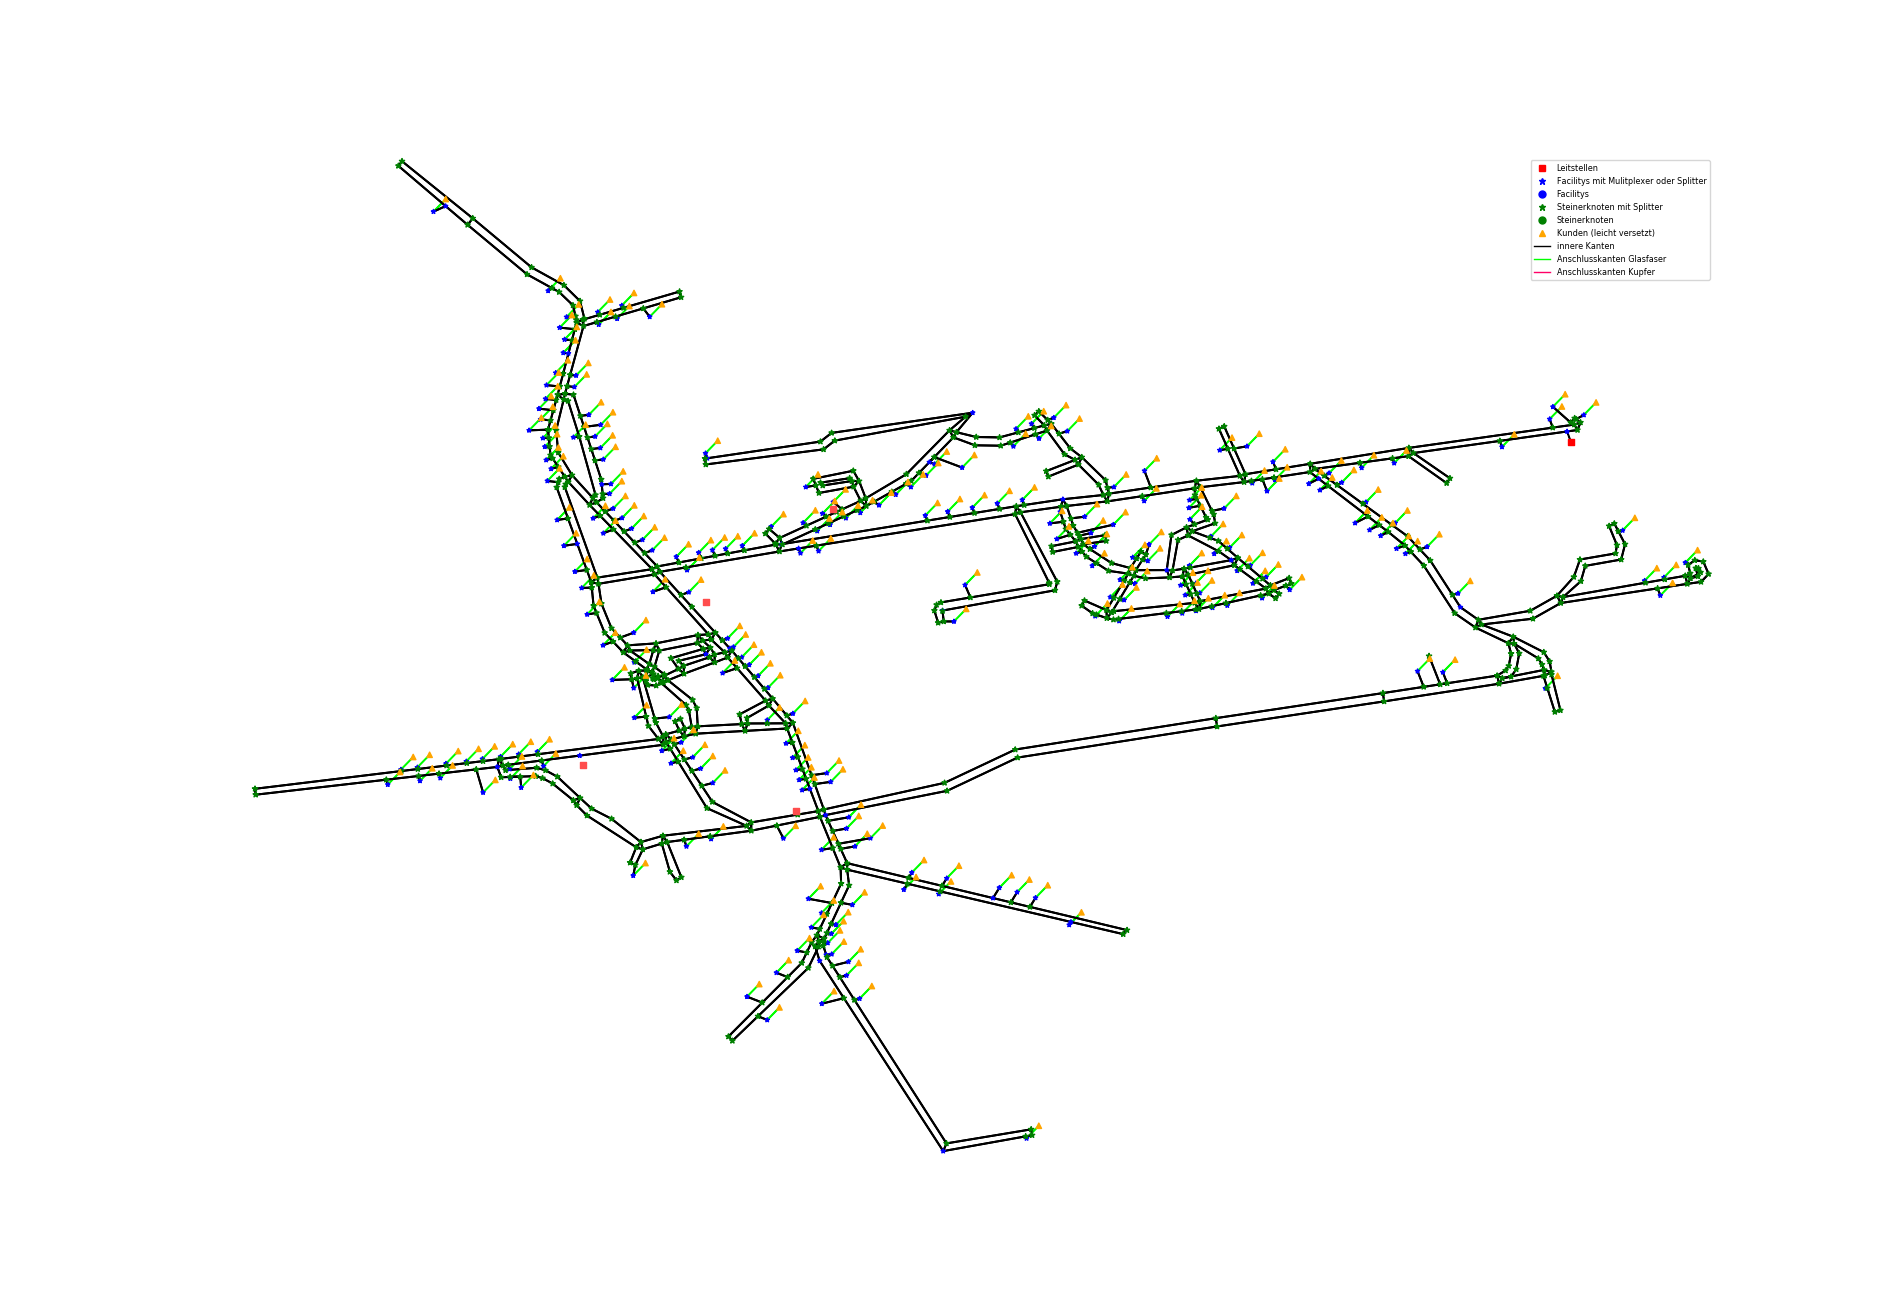
\includegraphics[width=1\textwidth]{./Bilder/P2MPG_Vehlefanz_demand1_duration0_upperbound}
			\caption{Obere Schranke der L\"osung des P2MPG Problems f\"ur \(a=4\) auf der Instanz Vehlefanz}
			\label{p2mpg_v_pic_ub}
		\end{minipage}
	\end{center}
\end{figure}

\begin{figure}[!htbp]
	\begin{center}
		\begin{minipage}{15.0cm}
			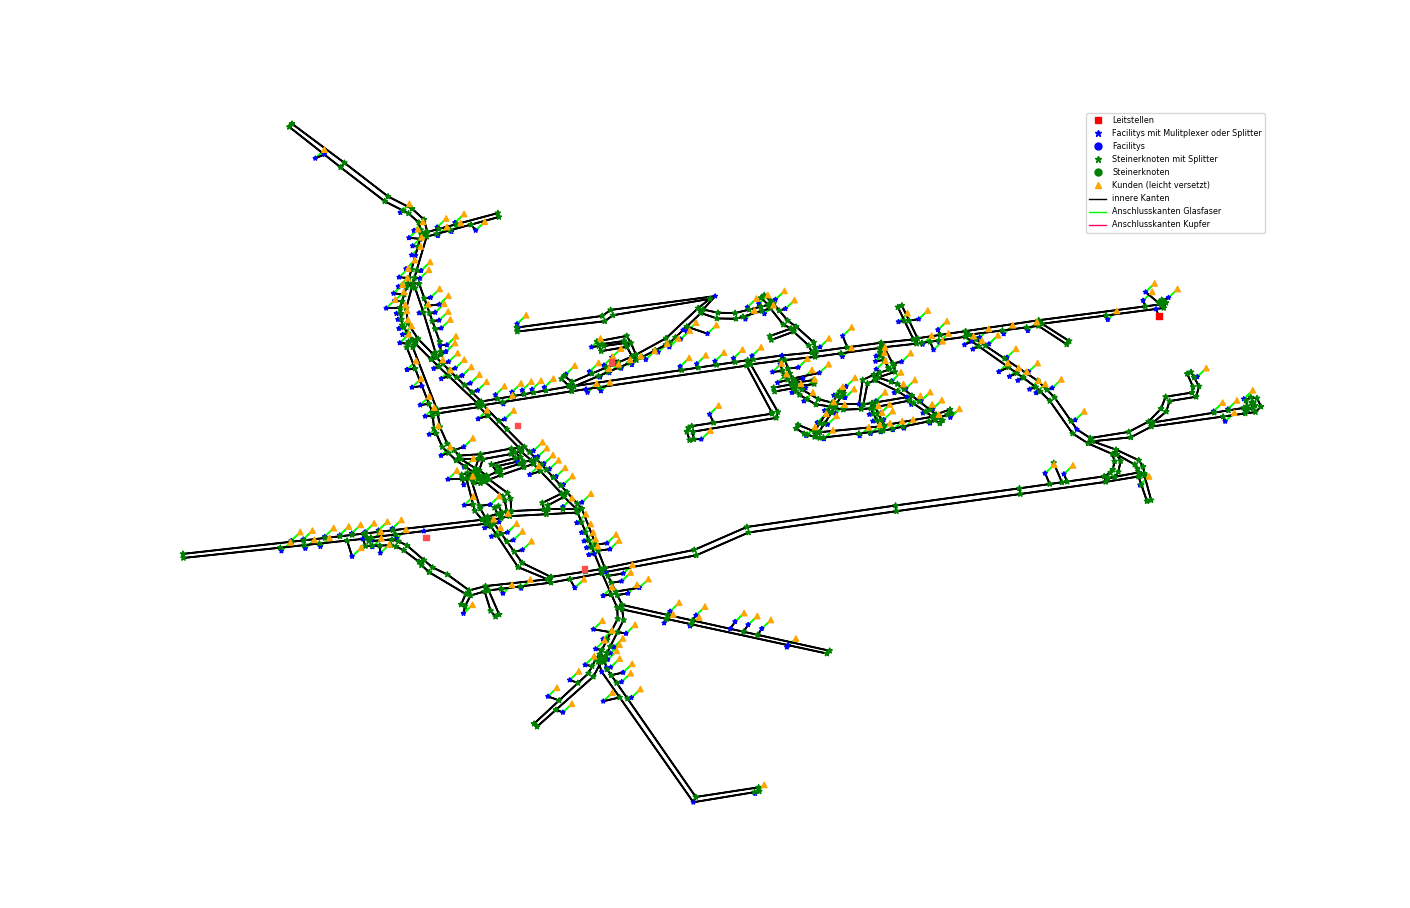
\includegraphics[width=1\textwidth]{./Bilder/P2MPG_Vehlefanz_demand1_duration0_SN16_upperbound}
			\caption{Obere Schranke der L\"osung des P2MPG Problems f\"ur \(a=16\) auf der Instanz Vehlefanz}
			\label{p2mpg_v_sn16_pic_ub}
		\end{minipage}
	\end{center}
\end{figure}

\begin{figure}[!htbp]
	\begin{center}
		\begin{minipage}{8.0cm}
			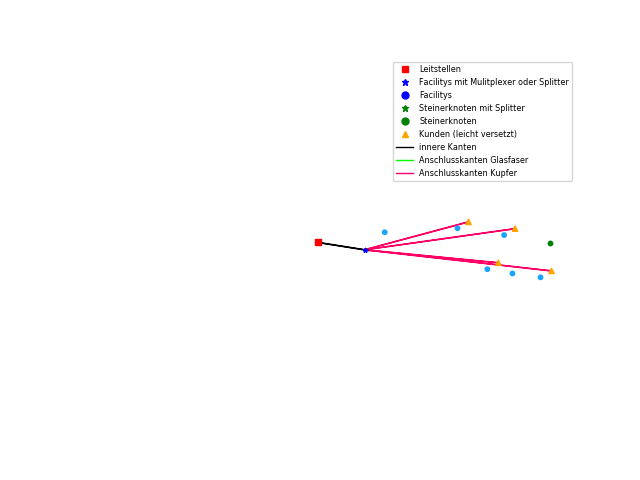
\includegraphics[width=1\textwidth]{./Bilder/P2MPGK_Naunyn_demand1_duration0}
			\caption{L\"osung des P2MPGK Problems mit \(a = 4\) auf der Instanz Naunyn}
			\label{p2mpgk_n_pic_sn4}
		\end{minipage}
	\end{center}
\end{figure}

\begin{figure}[!htbp]
	\begin{center}
		\begin{minipage}{8.0cm}
			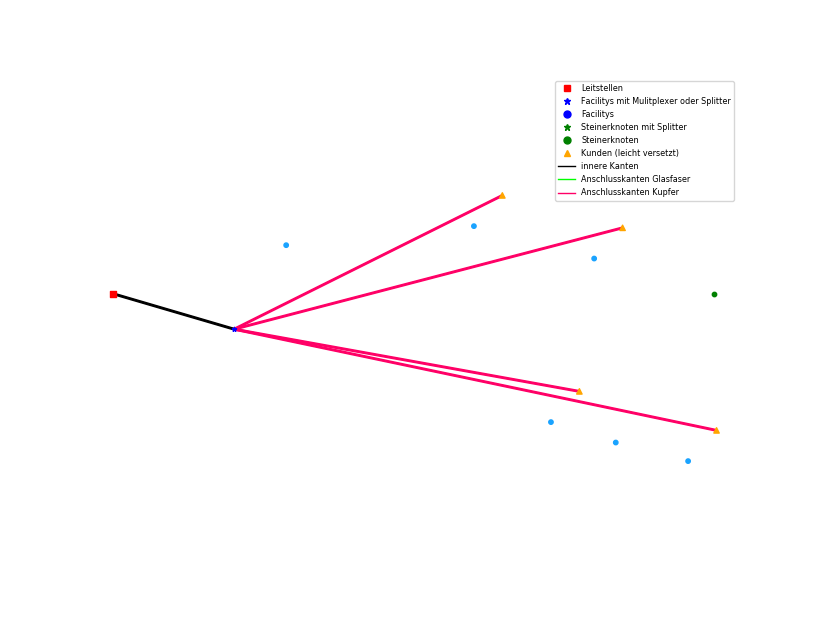
\includegraphics[width=1\textwidth]{./Bilder/P2MPGK_Naunyn_demand1_duration0_SN16}
			\caption{L\"osung des P2MPGK Problems mit \(a = 16\) auf der Instanz Naunyn}
			\label{p2mpgk_n_pic_sn16}
		\end{minipage}
	\end{center}
\end{figure}

\begin{figure}[!htbp]
	\begin{center}
		\begin{minipage}{15.0cm}
			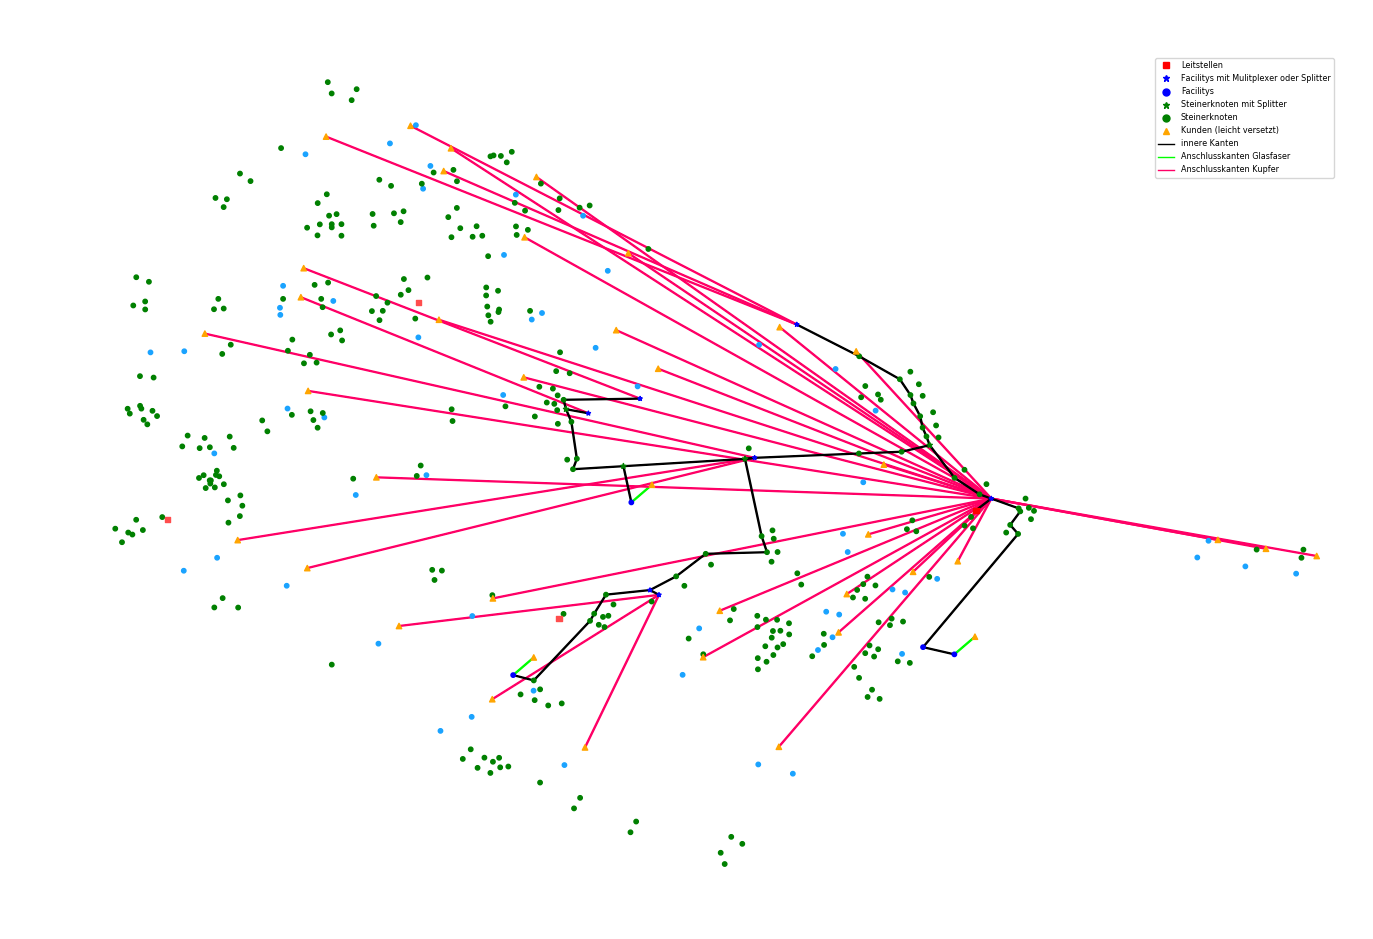
\includegraphics[width=1\textwidth]{./Bilder/P2MPGK_Berlin_demand1_duration0}
			\caption{L\"osung des P2MPGK Problems mit \(a = 4\) auf der Instanz Berlin}
			\label{p2mpgk_b_pic_sn4}
		\end{minipage}
	\end{center}
\end{figure}

\begin{figure}[!htbp]
	\begin{center}
		\begin{minipage}{15.0cm}
			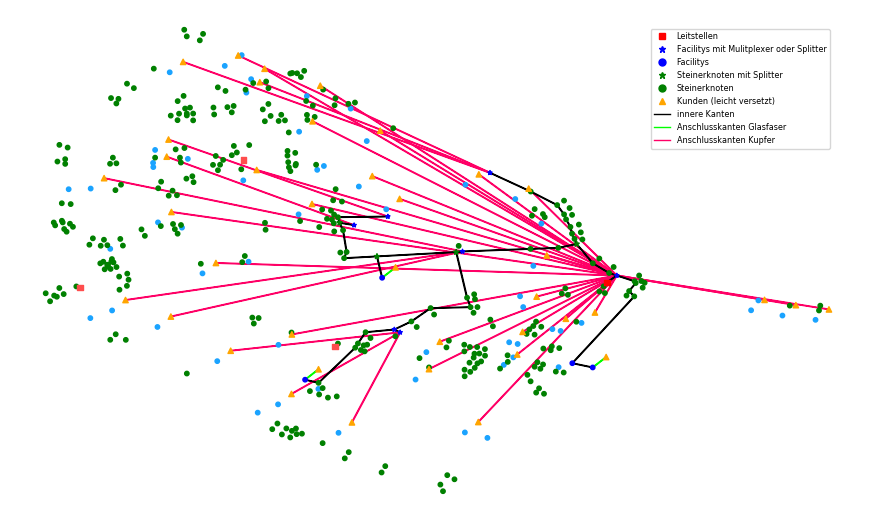
\includegraphics[width=1\textwidth]{./Bilder/P2MPGK_Berlin_demand1_duration0_SN16}
			\caption{L\"osung des P2MPGK Problems mit \(a = 16\) auf der Instanz Berlin}
			\label{p2mpgk_b_pic_sn16}
		\end{minipage}
	\end{center}
\end{figure}

\begin{figure}[!htbp]
	\begin{center}
		\begin{minipage}{15.0cm}
			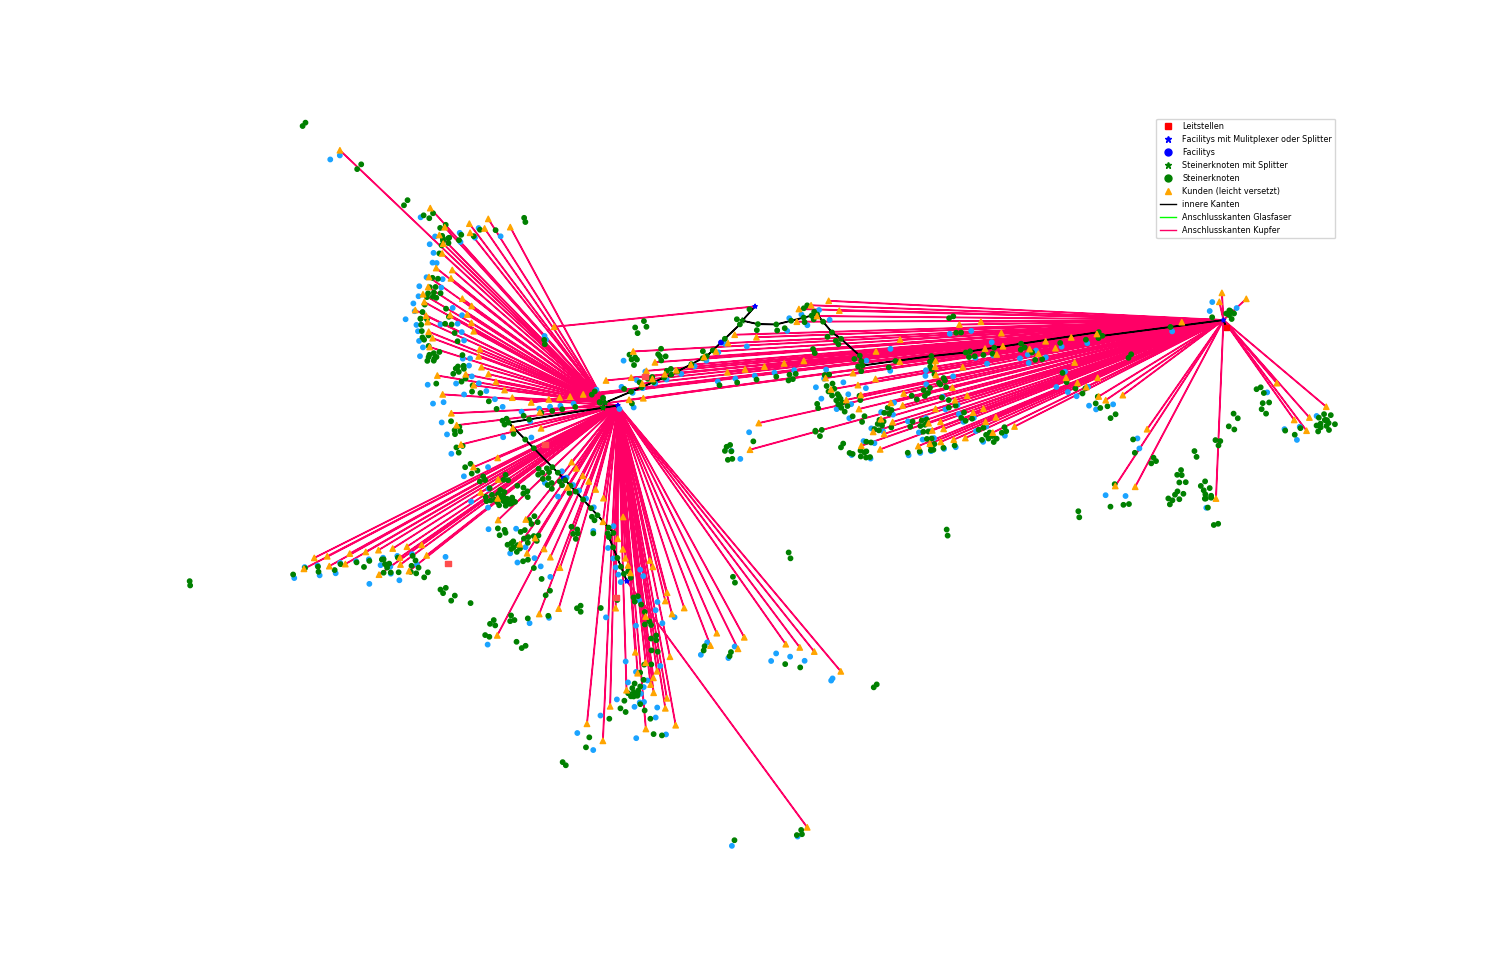
\includegraphics[width=1\textwidth]{./Bilder/P2MPGK_Vehlefanz_demand1_duration0}
			\caption{L\"osung des P2MPGK Problems mit \(a = 4\) auf der Instanz Vehlefanz}
			\label{p2mpgk_v_pic_sn4}
		\end{minipage}
	\end{center}
\end{figure}


\addcontentsline{toc}{section}{Abbildungsverzeichnis}
\clearpage
\section*{Anhang}
\subsection*{Steinerbaum Modell mit Flussformulierung}
\textbf{Gegeben:} Graph $G=(V,A)$, Menge an Terminalen $T \subseteq V $, Wurzel $r \in V$, Kostenfunktion $c:A \rightarrow \Q$\\
\textbf{Gesucht:} Teilgraph von $G$ (Steinerbaum), der alle Knoten aus $T$ verbindet und bei dem die Summe der Kosten minimal ist\\
\textbf{Entscheidungsvariablen:}\\
\begin{tabular}{lll}
	$y_{ij}^t \in \{0,1\}$ &$\forall ij \in A, t\in T $ & modelliert einen Fluss für jeden Terminal $t$ von der Wurzel $r$\\
	&& zum Terminal $t$\\
	$x_{ij} \in \{0,1\}$ & $\forall ij \in A$ &gibt an, ob die Kante $ij$ Teil des Steinerbaums ist ($x_{ij}=1$)\\
	&& oder nicht ($x_{ij}=0$)\\
\end{tabular}\\
\textbf{Modell:}
$\min \displaystyle\sum_{ij \in A} c_{ij} x_{ij} $
\begin{align}
\begin{array}{rcrcrcll}
\textrm{s.t.}  
&& &\displaystyle\sum_{ji \in A} y_{ji}^t - \displaystyle\sum_{ij \in A} y_{ij}^t& = & \left\{\begin{array}{rl} 
-1, & \text{falls } i=r\\ 
1, & \text{falls } i=t\\ 
0, & \text{sonst}\\ 
\end{array}
\right. & \forall t \in T & (1) \\
  &&& y_{ij}^t & \leq & x_{ij} & \forall ij \in A, t\in T & (2)\\
&&& y_{ij}^t & \in & \{0,1 \}& \forall ij \in A , t \in T& (3)\\
&&& x_{ij} & \in & \{0,1\}& \forall ij \in A & (4)\\
\end{array}
\label{SteinerbaumModel}
\end{align}

\subsection*{P2PGK mit Bedarfsfaktor}
Hier sind die Ergebnisse des P2PGK Problems mit Bedarfsfaktor $A_G$. Dabei ist $A_G$ die Anzahl der Kunden mit einem Glasfaseranschluss.

\begin{table}[h]
	\centering
	\begin{minipage}{.35\textwidth}
		\centering
		\begin{tabular}{c|c|c}
			\centering
			\(d\) & Kosten & $A_G$ \\	
			\hline
			1& 524.392 & 3 \\
			\(1,5\) & 709.412 & 10 \\
			2 & 834.472 & 15 \\
			\(2,5\) & 1.046.842 & 22 \\
			3 & 1.142.322 & 28 \\
			\(3,5\) & 1.152.122 & 28 \\
			4 & 1.174.552 & 30 \\
			\(4,5\) & 1.220.122 & 33 \\	
			5 & 1.220.122 & 33 \\
			$\infty$ &  1.388.562 & 39 \\
		\end{tabular}
		\caption{Lösung des P2PGK auf der Instanz Berlin mit veschiedenen Bedarfsfaktoren \(d\)}
		\label{P2PGK_Berlin_Bedarf}
	\end{minipage}
	\hspace{0.5cm}
	\begin{minipage}{0.35\textwidth}
		\centering
		\begin{tabular}{c|c|c}
			\centering
			$d$ & Kosten & $A_G$ \\	
			\hline
			$1$   &   647.608 & 0  \\
			$1,5$ &   647.608 & 0  \\
			$2$   &   826.768 & 3  \\
			$2,5$ &   907.508 & 7  \\
			$3$   & 1.274.782 & 15 \\
			$3,5$ & 1.924.742 & 40 \\
			$4$   & 2.137.362 & 47 \\
			$4,5$ & 2.325.942 & 56 \\
			$5$   & 2.350.572 & 57 \\
			$\infty$ & 7.791.258 & 238 \\ 
		\end{tabular}
		\caption{Lösung des P2PGK auf der Instanz Vehlefanz mit veschiedenen Bedarfsfaktoren $d$}
		\label{P2PGK_Vehlefanz_Bedarf}
	\end{minipage}
\end{table}
\vspace{0.5cm}

\subsection*{P2PGK mit Profit}
Hier sind die Ergebnisse des P2PGK Problems mit Profit. Dabei ist $A_G$ die Anzahl der Kunden mit einem Glasfaseranschluss.

\begin{table}[!htbp]
	\centering
	\begin{tabular}{c|c|c}
		\centering
		Jahre & Kosten & $A_G$ \\	
		\hline
		$0$   	 &  397.662& 0  \\
		$10$ 	&  382.062 & 0  \\
		$20$   	&  366.462  & 0  \\
		$30$    &  350.862 & 0  \\
		$40$    &  335.262  & 0 \\
	\end{tabular}
	\caption{Ergebnisse des P2PGK mit Profit f\"ur Naunyn}
	\label{P2PGKProfitN}
\end{table}

\begin{table}[!htbp]
	\centering
	\begin{tabular}{c|c|c}
		\centering
		Jahre & Kosten & $A_G$ \\	
		\hline
		$0$   	 &  524.392 & 3  \\
		$10$ 	&   366.112& 3  \\
		$20$   	&   207.832 & 3  \\
		$30$    &   49.552 & 3  \\
		$40$    & $-111.448$ & 4 \\
	\end{tabular}
	\caption{Ergebnisse des P2PGK mit Profit f\"ur Berlin} 
	\label{P2PGKProfitB}
\end{table}

\begin{table}[!htbp]
	\centering
	\begin{tabular}{c|c|c}
		\centering
		Jahre & Kosten & $A_G$ \\	
		\hline
		$0$   	 & 647608  &0  \\
		$10$ 	&  426.328 & 0  \\
		$20$   	&  205.048  & 0  \\
		$30$    & $-16.232$& 0  \\
		$40$    &  $-237.512$ & 0 \\
	\end{tabular}
	\caption{Ergebnisse des P2PGK mit Profit f\"ur Vehlefanz}
	\label{P2PGKProfitV}
\end{table}

\vspace{3cm}

\subsection*{P2MPGK mit Bedarfsfaktor}
Hier sind die Ergebnisse des P2MPGK Problems mit Bedarfsfaktor $d$. Dabei ist $A_G$ die Anzahl der Kunden mit einem Glasfaseranschluss.
\begin{table}[!htbp]
	\centering
		\begin{tabular}{c|c|c}
	\centering
	$d$ & Kosten & $A_G$ \\	
	\hline
	$1$   	 &  397.622 & 0  \\
	$1,5$ 	&   $427.553,11$  & 2  \\
	$2$   	&   $427.553,11$ & 2  \\
	$2,5$   	&   $427.553,11$ & 2  \\
	$3$    &   $427.553,11$ & 2  \\
	$3,5$   	&   $445.743,11$ & 3  \\
\end{tabular}
	\caption{Ergebnisse des P2MPGK mit Bedarfsfaktor $d$ f\"ur Naunyn}
	\label{P2MPGKBedarfN} 
\end{table}

\begin{table}[!htbp]
			\centering
			\begin{tabular}{c|c|c}
				\centering
				$d$ & Kosten & $A_G$ \\	
		\hline
	$1$   	 &  474.909,28 & 3  \\
	$1,5$ 	&  543.177,46   & 10  \\
	$2$   	& 572.319,28 & 15  \\
	$2,5$  & 621.717,47  & 22  \\
	$3$    &  653.629,29  & 28  \\
			\end{tabular}
			\caption{Ergebnisse des P2MPGK mit Bedarfsfaktor $d$ f\"ur Berlin} 
			\label{P2MPGKBedarfB}
\end{table}

% [[1, 0, 'B_551', 474909.2763945444, 3, False], [1.5, 0, 'B_551', 543177.4626992824, 10, False], [3, 0, 'B_551', 653629.2929971206, 28, False], [2, 0, 'B_551',572319.2843613572, 15, False]]


\begin{table}[!htbp]
	\centering
	\begin{tabular}{c|c|c}
		\centering
		$d$ & Kosten & $A_G$ \\	
		\hline
		$1$   	 &  \(587.503,28\) & 0  \\
		$1,5$ 	&   $587.503,28$  & 0  \\
		$2$   	&   $615.147,07$ & 3 \\
		$2,5$   	&   $628.724,59$ & 7 \\
		$3$    &   $677.145,90$ & 14 \\
		$3,5$   	&   $756.123,57$ & 40 \\
	\end{tabular}
	\caption{Ergebnisse des P2MPGK mit Bedarfsfaktor $d$ f\"ur Vehlefanz} 
	\label{P2MPGKBedarfV}
\end{table}

\vspace{5cm}

\subsection*{P2MPGK mit Profit}
Hier sind die Ergebnisse des P2MPGK Problems mit Profit. Dabei ist $A_G$ die Anzahl der Kunden mit einem Glasfaseranschluss.

\begin{table}[!htbp]
	\centering
	\begin{tabular}{c|c|c}
		\centering
		Jahre & Kosten & $A_G$ \\	
		\hline
		$0$   	 & \(397.662\) & 0  \\
		$10$ 	&  \(382.062\) & 0  \\
		$20$   	&  \(366.462\)  & 0  \\
		$30$    &  \(350.862\) & 0  \\
		$40$    &  \(332.513,11\)  & 2 \\
	\end{tabular}
	\caption{Ergebnisse des P2MPGK mit Profit f\"ur Naunyn} 
	\label{P2MPGKProfitN}
\end{table}

\begin{table}[!htbp]
	\centering
	\begin{tabular}{c|c|c}
		\centering
		Jahre & Kosten & $A_G$ \\	
		\hline
		$0$   	 &  \(474.909,28\) & 3  \\
		$10$ 	&  \(316.320,18\) & 5  \\
		$20$   	&   \(145.851,10\) & 7  \\
		$30$    &   $ -34.146,17$	& 15  \\
		$40$    & $-235.002,54$ &  24 \\
	\end{tabular}
	\caption{Ergebnisse des P2MPGK mit Profit f\"ur Berlin}
	\label{P2MPGKProfitB}
\end{table}

\begin{table}[!htbp]
	\centering
	\begin{tabular}{c|c|c}
		\centering
		Jahre & Kosten & $A_G$ \\	
		\hline
		$0$   	 & $587.503,28$ &0  \\
		$10$ 	& $366.233,28$ & 0  \\
		$20$   	&  $144.762,04$  & 1  \\
		$30$    &  $-81.400,37$ & 12 \\
	\end{tabular}
	\caption{Ergebnisse des P2MPGK mit Profit f\"ur Vehlefanz} 
	\label{P2MPGKProfitV}
\end{table}

\addcontentsline{toc}{section}{Anhang}


\end{document}
